\documentclass[letterpaper,9pt,twocolumn,twoside,]{pinp}

%% Some pieces required from the pandoc template
\providecommand{\tightlist}{%
  \setlength{\itemsep}{0pt}\setlength{\parskip}{0pt}}

% Use the lineno option to display guide line numbers if required.
% Note that the use of elements such as single-column equations
% may affect the guide line number alignment.

\usepackage[T1]{fontenc}
\usepackage[utf8]{inputenc}

% pinp change: the geometry package layout settings need to be set here, not in pinp.cls
\geometry{layoutsize={0.95588\paperwidth,0.98864\paperheight},%
  layouthoffset=0.02206\paperwidth, layoutvoffset=0.00568\paperheight}

\definecolor{pinpblue}{HTML}{185FAF}  % imagecolorpicker on blue for new R logo
\definecolor{pnasbluetext}{RGB}{0,101,165} % default in pinp.cls


\usepackage{booktabs}
\usepackage{longtable}
\usepackage{array}
\usepackage{multirow}
\usepackage{wrapfig}
\usepackage{float}
\usepackage{colortbl}
\usepackage{pdflscape}
\usepackage{tabu}
\usepackage{threeparttable}
\usepackage{threeparttablex}
\usepackage[normalem]{ulem}
\usepackage{makecell}
\usepackage{xcolor}

\title{Understanding the relationship between the El Niño Southern
Oscillation and Degree Heating Weeks across the Great Barrier Reef}

\author[a]{Charley Johnson}
\author[b]{Chengxi Duan}
\author[c]{Fiona Li}
\author[d]{Hussain Karimi}
\author[e]{Imane Lattab}
\author[f]{Kunlei Zhang}
\author[g]{Oscar Lo Lu}
\author[h]{Tingzhao Dai}

  \affil[a]{520482628}
  \affil[b]{530005104}
  \affil[c]{520404414}
  \affil[d]{530516493}
  \affil[e]{530318646}
  \affil[f]{520377451}
  \affil[g]{530528429}
  \affil[h]{510343068}

\setcounter{secnumdepth}{0}

% Please give the surname of the lead author for the running footer
\leadauthor{}

% Keywords are not mandatory, but authors are strongly encouraged to provide them. If provided, please include two to five keywords, separated by the pipe symbol, e.g:
 \keywords{  enso |  great barrier reef |  gbr |  ocean temperature  }  

\begin{abstract}
Increasingly frequent and extreme El Niño Southern Oscillation (ENSO)
events driven by climate change have heightened the need to protect
vulnerable ecosystems such as the Great Barrier Reef (GBR). However, the
specific relationship between ENSO events and thermal stress across the
reef over time is insufficiently understood. This study aims to address
this knowledge gap and examine the appropriateness of using ENSO as an
indicator of thermal stress in the GBR. Findings will inform government
bodies such as the Great Barrier Marine Park Authority (GBRMPA) during
decision-making regarding the implementation of reef protective
strategies. This study aimed to predict temperature using the Southern
Oscillation Index (SOI) as an ENSO indicator, as well as other temporal
and spatial variables. Using historical time series data in the GBR,
four models were fitted and evaluated and the Generalised Additive Model
(GAM) was selected. ENSO was found to have a significant effect on
Degree Heating Weeks (DHW), sea-surface temperature (SST) and SST
anomalies (SSTA). El Niño phases were associated with greater thermal
stress. Additionally, the effect of ENSO on temperature differed across
the continental shelves. These findings suggest that ENSO may be a
useful indicator of thermal stress events that increase the risk of
bleaching events.These findings suggest that ENSO phases could be
implemented into temperature forecasting, as well as monitored according
to spatial, temporal and seasonal changes.
\end{abstract}

\dates{This version was compiled on \today} 


% initially we use doi so keep for backwards compatibility
% new name is doi_footer
\doifooter{\url{https://github.com/DipsyCdua/reef}}

\pinpfootercontents{Reef03 MARS/DATA3888 2025, The University of Sydney}

\begin{document}

% Optional adjustment to line up main text (after abstract) of first page with line numbers, when using both lineno and twocolumn options.
% You should only change this length when you've finalised the article contents.
\verticaladjustment{-2pt}

\maketitle
\thispagestyle{firststyle}
\ifthenelse{\boolean{shortarticle}}{\ifthenelse{\boolean{singlecolumn}}{\abscontentformatted}{\abscontent}}{}

% If your first paragraph (i.e. with the \dropcap) contains a list environment (quote, quotation, theorem, definition, enumerate, itemize...), the line after the list may have some extra indentation. If this is the case, add \parshape=0 to the end of the list environment.


\section{Introduction}\label{introduction}

The Great Barrier Reef (GBR) is the largest world Heritage Listed Area
globally and highly biodiverse, supporting many industries related to
fisheries, shoreline protection and reef tourism \citet{Fabricius2000}.
Over recent decades, thermal stress events have increased in both
frequency and intensity, leading to coral bleaching events across the
GBR \citet{vanWoesik2022}. This study aims to examine how ENSO affects
temperatures on the GBR, and whether this effect differs with different
depth regions of the reef (inner, mid, and outer shelf). Understanding
the relationship between ENSO and accumulated heat stress (in this
study, DHW) is essential for informing the appropriateness of using ENSO
as a predictor of coral bleaching and developing effective policies and
legislations to protect the GBR.

\subsubsection{El Niño Southern Oscillation
(ENSO)}\label{el-niuxf1o-southern-oscillation-enso}

ENSO is a natural climate oscillation measured by the Southern
Oscillation Index (SOI), with El Niño (negative SOI, weaker trade winds)
and La Niña (positive SOI, stronger trade winds) phases impacting
Australian weather differently (\emph{figure 1}) \citet{Lough1994}. El
Niño's weaker winds lead to hotter conditions in north-east Australia,
while La Niña's stronger trade winds bring wetter conditions
(\emph{figure 1}) \citet{McGowanTheobald2017}.

\begin{figure}[H]
\centering
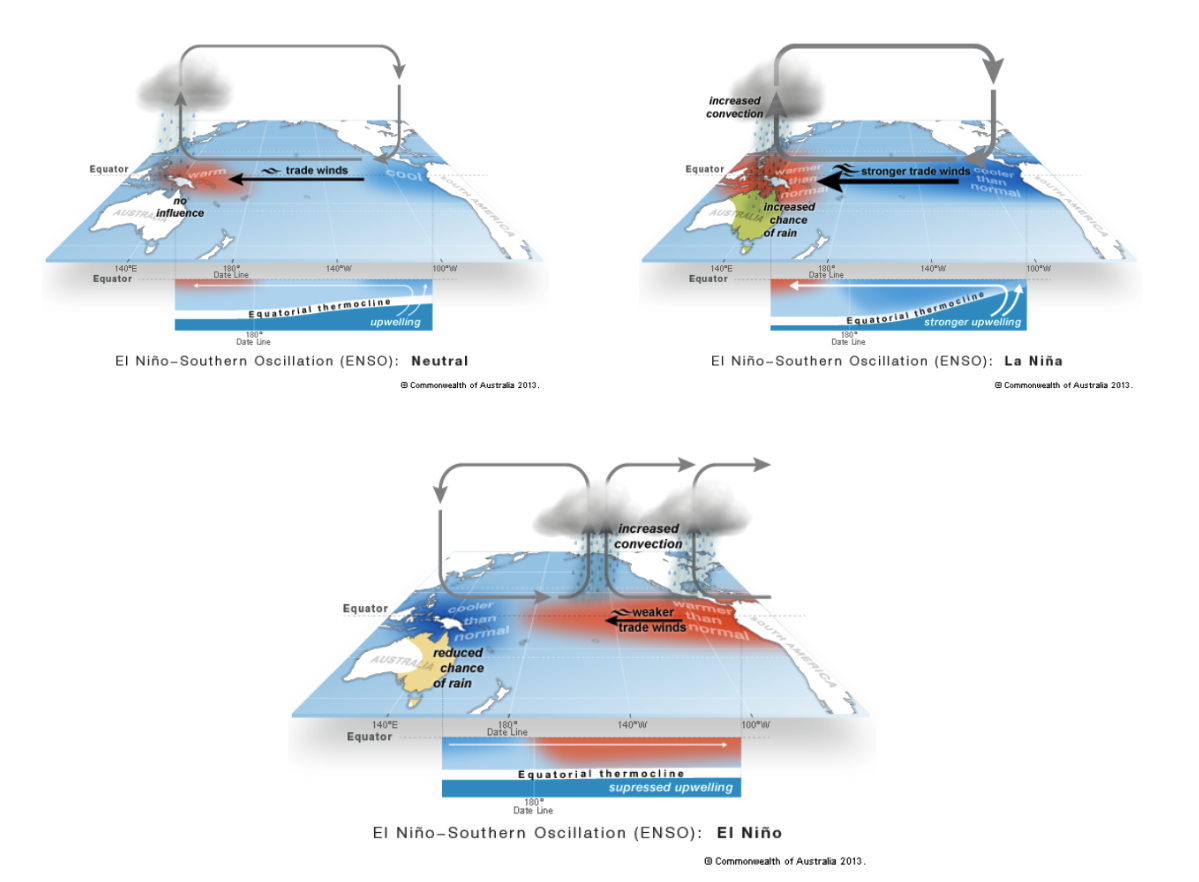
\includegraphics[width=0.5\textwidth]{report_images/enso_cycles.png}
\caption{Neutral, La Nina, and El Nino ENSO phase, Bureau of Meteorology}
\end{figure}

\subsubsection{Degree Heating Weeks
(DHW)}\label{degree-heating-weeks-dhw}

Degree Heating Weeks is a measure of the intensity and duration of
thermal stress, with 4 °C-weeks indicating significant coral bleaching,
and 8 °C-weeks indicative of significant mortality
\citet{NOAA_CRW_Methodology}. It is a valuable measurement of thermal
stress as it indicates cumulative temperature anomalies.

The frequency and severity of ENSO fluctuations has increased since the
1960s causing stronger El Niño and La Niña events \citet{Cai2023}. This
is expected to increase across all future emission scenarios, leading to
increases in SST anomalies \citet{Cai2022}. Understanding the
relationship between ENSO and DHWs may allow an identification of areas
that are more at risk in specific phases, or show which sections of the
reef are more susceptible to changes in SST. The models aim to explore
the impacts of ENSO spatially and temporally across the GBR to inform
decision making and policies in the context of increasingly variable
future predictions.

This study is supported by the development of a Shiny app designed to
support the Great Barrier Reef Marine Park Authority (GBRMPA) in making
informed decisions surrounding policies targeted towards coral health
and protection.

\section{Methods}\label{methods}

\subsection{Data Collection}\label{data-collection}

The data collection process was thorough and extensive, beginning with
an initial exploratory review of multiple potential datasets relevant to
ocean temperature, ENSO and other climate variables across the GBR. We
initially considered site-level meteorological data from published
databases, however, these were limited in both spatial and temporal
resolution. Ultimately, high-resolution satellite temperature data from
the \citet{NOAA_CRW2024} was chosen as it provides consistent, spatially
extensive coverage of the GBR from 1985-2025 and across the Coral Sea.

\subsection{Data Cleaning \&
Preprocessing}\label{data-cleaning-preprocessing}

The NOAA data was retrieved as monthly NetCDF files with spatial and
daily temperature data for three measures; DHW, SST and SSTA. The
following data cleaning pipeline was followed using R (and sometimes
Python) to transform raw data into one dataset with monthly average
temperature of the GBR:

\begin{enumerate}
\def\labelenumi{\arabic{enumi}.}
\item
  \emph{Extract raster data and pivot longer}: longitude, latitude and
  daily temperature data as extracted and reshaped to long format.
\item
  \emph{Remove land points}: null marine temperature data corresponded
  to land values, which were dropped.
\item
  \emph{Aggregate monthly means}: daily data was summarised into monthly
  averages for every point, then dataframes were joined by year (with
  duplicate rows for date).
\item
  \emph{GBR data}: using the \citet{GBRMPA2017} shape files, we limited
  the data to only the GBR region.
\item
  \emph{Merge across variables and time}: separate yearly files for
  temperature were merged across DHW, SST and SSTA by location and time,
  then unified to one single dataset containing 1987-2025 GBR data.
\item
  \emph{Continental Shelf}: using bathymetry depth data
  \citet{GA_HIGHRES_BATHY}, the GBR was divided into three continental
  shelf zones (inner shelf = 0-20 m, mid shelf = 20-40 m, outer shelf =
  40-90 m) defined by previous research \citet{Belperio1983}
  \citet{Maxwell1968}. These newly defined continental shelf boundaries
  were saved as shape files and used in our shiny app.
\item
  \emph{SOI cleaning \& integration}: \citet{NOAA_SOI2025} text file was
  cleaned in python. SOI monthly SOI anomalies were extracted, defined
  as SOI variations from the 1990-2010 period. SOI data was merged into
  the full reef temperature dataframe.
\end{enumerate}

The cleaned data was exported as a CSV file with the dimensions
{[}5,195,088 × 11{]}. The variables are;

```mean\_dhw'', ``mean\_sst'', ``mean\_ssta'', ``date'', ``lon'',
``lat'', ``shelf'', ``soi\_anomaly'', ``year'', month''\,``

Downsizing the daily time series to monthly averages was a carefully
considered tradeoff prioritising spatial resolution. The use of shelf
zones also summarises the spatial variation and will allow the models to
explore the effects of SOI spatially.

\subsection{Model Development}\label{model-development}

The aim of this study was to predict 3 different temperature measures
(DHW, SST and SSTA) using SOI anomalies, continental shelf, month, year
and the interactions between SOI and all predictors. SOI was chosen as
the index for ENSO as it is an extensive dataset that is widely used for
recording ENSO. Continental shelf zone was chosen as a predictor
variable as different water depths are known to behave differently with
respect to temperature. For example, deeper waters are expected to
experience more cold water mixing and stratification than shallow
waters, potentially impacting the capacity for heat accumulation
\citet{DorrellLloyd2022}. Four different model approaches were
evaluated.

\subsubsection{1. Linear Regression}\label{linear-regression}

To evaluate the suitability of linear regression (LR) for predicting
coral reef thermal stress indicators (DHW, SST, and SSTA), linear
assumptions were assessed (see \textbf{Appendix A} for Q-Q and residual
plots). While the SSTA model satisfied normality and homoscedasticity,
DHW and SST showed substantial deviations and heteroscedastic residuals.
We proceeded under the Central Limit Theorem (CLT) due to sufficient
sample size. However, independence is uncertain due to repeated temporal
observations. Correlation matrix and VIF (\textbf{Appendix A}) were used
to check multicollinearity. To determine predictor order, four model
selection approaches were used: AIC, BIC, forward, and backward
selection. Models were compared using in-sample and out-of-sample Mean
Absolute Error (MAE), Root Mean Squared Error (RMSE) and \(R^2\). Final
selection was based on overall performance: BIC was best for DHW and
SST, forward selection for SSTA. While LR captured general trends and
supported interpretation, it struggled with non-linear and temporally
structured data patterns (\textbf{Appendix B}).

\subsubsection{2. Mixed Effects Model}\label{mixed-effects-model}

Mixed effects models (MEM) is another linear model approach that will
account for SOI anomalies as a fixed effect, while temporal (year,
month) and spatial (reef shelf) variables were included as random
effects to isolate the effect of ENSO. The same assumptions were checked
for the LR apply to the MEMs (\textbf{Appendix A}). After evaluating the
performance on the test data, it was found that the SSTA model performed
better than SST and DHW (See \emph{figure 2} for values). Across all the
models, continental shelf was a significant random effect where outer
reefs were consistently warmer. SOI anomaly had a strong negative effect
on SSTA, highlighting its relevance for predicting thermal stress. See
\textbf{Appendix C} for detailed model performance. However, MEMs are
limited by their inability to fully account for temporal autocorrelation
and the nonlinear effects of temperature and SOI (which was flagged
during the assumption checking).

\subsubsection{3. Random Forest
Regression}\label{random-forest-regression}

The RF model appeared to be more suitable than MEM and LR due to its
ability to capture these non-linear relationships. To manage the high
computational cost, a 10-fold cross-validation was applied to smaller
yearly samples, each representing 1\% of the full dataset and
hyperparameter tuning was done manually. An optimal number of 150 trees
and \(mtry = 2\) balanced predictive performance and efficiency.
Residual plots showed more reliable predictions than LR and MEM, but the
wide scatter indicates the model's predictive limitations. (See
\textbf{Appendix D}). RF performed best on SST based on \(R^2\),
capturing much of the variance across years. For SSTA, performance was
highest in terms of MAE and RMSE, suggesting a weak association between
SOI anomaly and SSTA. This indicates that positive SOI anomalies may
contribute to warmer sea surface anomalies. This result supports the
model's ability to reflect known climatic influences despite some
predictive limitations.

\subsubsection{4. Generalised Additive
Model}\label{generalised-additive-model}

To model nonlinear relationships between SOI and marine temperature
across continental shelves, Generalised Additive Models (GAMs) were
fitted. These allowed flexible estimation of continuous predictors,
inclusion of categorical variables and interactions - particularly with
SOI. The aim was both to understand individual effects and to develop a
useful forecasting tool. Therefore, two pursued GAM modelling approaches
were implemented. First, global GAMs were trained on pre-2015 data,
reserving post-2015 observations for evaluation. \texttt{month} was
modelled using a cyclic cubic spline
(\texttt{s(month,\ bs\ =\ "cc",\ k\ =\ 12)}), with shelf zone as a fixed
effect. Interaction smooths included
\texttt{ti(soi\_anomaly,\ by\ =\ shelf)} for spatial variation in SOI
effects, \texttt{ti(soi\_anomaly,\ year)} for long-term trends, and
\texttt{ti(soi\_anomaly,\ month,\ bs\ =\ c("tp",\ "cc"))} for seasonal
modulation (see \textbf{Appendix E} for outputs). The second approach
was geared towards the Shiny app predictive tool. A rolling-origin
forecast validation was implemented to assess the predictive performance
over time (implemented for the Shiny predictive tool). The model was
refitted each year with cumulative historical data, and forecasts were
made for the following year. This approach mimics real-time application
and tests temporal generalisability, identifying which years the
predictions were problematic - potentially signaling years where SOI and
temperature were more correlated (See \textbf{Appendix F} for yearly
performance).

\subsection{Model Selection}\label{model-selection}

All four models were evaluated using MAE, RMSE and \(R^2\). These were
summarised across the four models (See \emph{figure 2}). Overall, GAMs
consistently outperformed LR and MEM across all DHW, SST and SSTA,
indicating better generalisation. GAMs were also preferred over LR and
MEM due to their flexibility in capturing nonlinear relationships
without requiring strong parametric assumptions. Unlike RF, which also
handle nonlinearity well but are hard to interpret meaningfully, GAMs
allow visual and statistical interpretation of smooth functions. This
interpretability was crucial for understanding how SOI varied by season,
time and shelf zone. A key limitation of GAMs is the assumption of
stationarity in smooth functions outside the training period. This may
limit extrapolation and long-term forecasting reliability. To mitigate
this, we implemented a rolling forward validation approach, where models
were re-fit on all years prior to the target year. This strategy allowed
us to assess performance across time while minimising information
leakage. The random forest model was also not selected due to its
significant computational costs when using large data (millions of
rows), hence additionally efficiency was a factor in our decision. Full
model specifications and smooth term plots are provided in
\textbf{Appendices E, G, and H}.

\begin{figure}[H]

{\centering 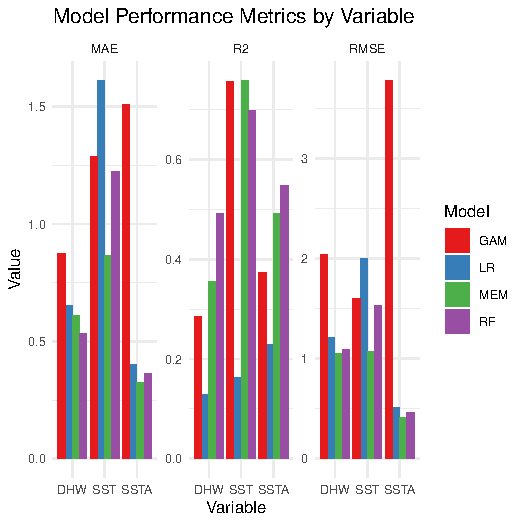
\includegraphics[width=1\linewidth,height=200px]{Reef03_FinalReport_files/figure-latex/unnamed-chunk-2-1} 

}

\caption{Figure 2 - Model Evaluation using Performance Metrics}\label{fig:unnamed-chunk-2}
\end{figure}

\section{Results}\label{results}

All three global GAMs revealed significant nonlinear effects of the SOI
anomaly, year, and month on temperature responses (\(p < 0.001\)). For
\emph{SST}, the model explained 74.1\% of deviance (adj. \(R^2\) =
0.758), with a strong interaction between SOI and shelf zone O (p
\textless{} 0.001), indicating spatially heterogeneous ENSO effects.
\emph{DHW} and \emph{SSTA} models explained 65.2\% and 37.5\% of
deviance respectively, with similarly strong temporal smooths and modest
spatial interactions. Parametric effects showed that outer shelf areas
consistently differed from inner shelf areas, particularly for
\emph{SST}. Full summaries and smooth plots are detailed in
\textbf{Appendix E, G and H}. The models revealed distinct response
patterns across temperature metrics (refer to Appendix E and F). First,
DHW exhibited a steep increase under strong negative SOI anomalies.
Conversely, DHW remained near zero across neutral and positive SOI
values (See \emph{figure 3}). Second, SST showed a modest U-shaped
relationship with SOI anomaly, with slightly elevated SSTs observed
under both El Niño and La Niña conditions. The lowest SST values
occurred near neutral SOI values (See \emph{figure 4}). However, the
overall effect size was small and confidence intervals widened at the
distribution tails. Finally, SSTA appeared to increase non-linearly with
decreasing SOI anomaly (See \emph{figure 5}).

\begin{figure}[H]
\centering
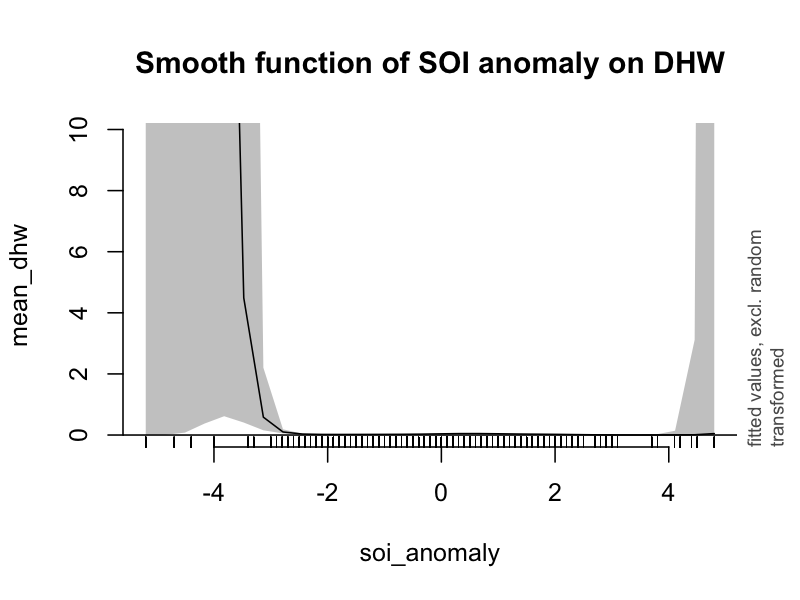
\includegraphics[width=0.5\textwidth]{report_images/dhw_soi.png}
\caption{DHW: SOI Smoothed Function}
\end{figure}

\begin{figure}[H]
\centering
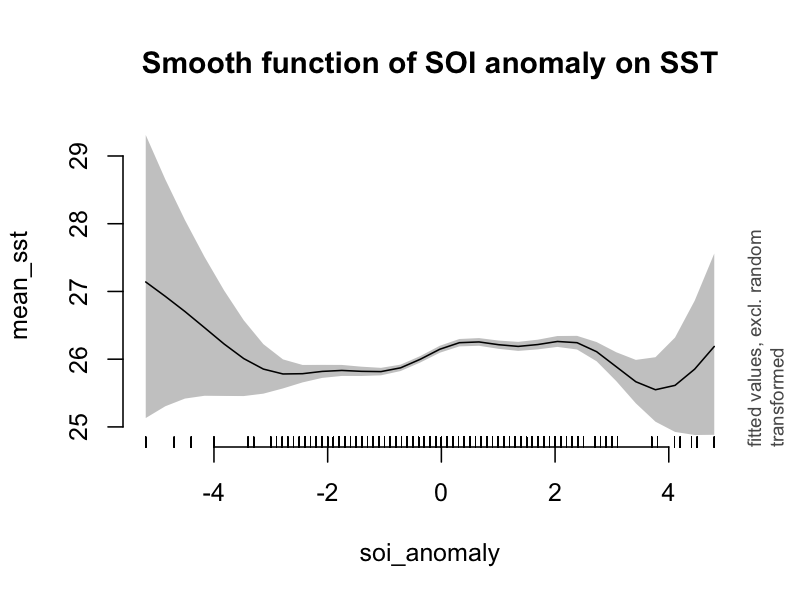
\includegraphics[width=0.5\textwidth]{report_images/sst_soi.png}
\caption{SST: SOI Smoothed Function}
\end{figure}

\begin{figure}[H]
\centering
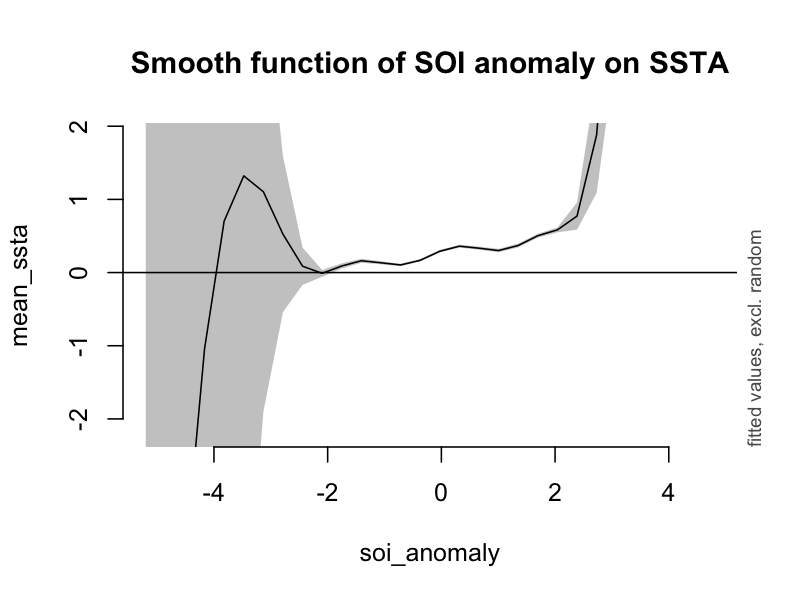
\includegraphics[width=0.5\textwidth]{report_images/ssta_soi.png}
\caption{SSTA: SOI Smoothed Function}
\end{figure}

\section{Shiny Application}\label{shiny-application}

Our Shiny application enables users to explore how ENSO variability
relates to sea-surface temperature across the GBR (refer to
\textbf{Appendix I}). It features four main tabs: \textbf{Introduction,
Heat Map of the GBR, ENSO vs Temperature}, and \textbf{Predictions}.

The \textbf{Introduction} tab outlines the scientific context and
purpose of the app.

In the \textbf{Heat Map} tab, users can select a year (1987--2024) and
temperature variable (DHW, SST, or SSTA) to visualise annual spatial
patterns across the reef. Bathymetric shelf zones (Inner, Mid, Outer)
can be toggled, and users can compare two years side-by-side to identify
historical trends or hotspots.

The \textbf{ENSO vs Temperature} tab links monthly SOI values with reef
temperatures. Users can select a year to see how DHW, SST, or SSTA
varies by month and shelf zone.

Finally, the \textbf{Predictions} tab presents GAM outputs. Users can
compare predicted vs observed temperatures for a selected year and
variable, with shelf overlays for added context. A summary below the
maps highlights how SOI and other predictors influence reef
temperatures, offering insights into thermal risk and model performance.

\section{Discussion}\label{discussion}

The results of the GAMs suggest that El Niño phases are associated with
significant thermal stress accumulation while La Niña and neutral phases
are minimally related to thermal stress. This aligns with existing
evidence that El Niño causes warmer conditions in eastern Australia due
to reduced cloud cover, greater solar radiation and reduced mixing of
deep, cold water \citet{McGowanTheobald2023}. Similarly, SST was greater
during El Niño phases, but was also greater during La Niña phases, as
was SSTA. High SST and SSTA during a La Niña, although counterintuitive,
aligns with recent evidence of coral bleaching during the 2021-2022 La
Niña event \citet{McGowanTheobald2023}. This heat stress observed in La
Niña is likely a result of anomalous atmospheric circulation patterns
that brought weather conditions similar to an El Niño phase
\citet{Gillett2023}. It is unclear whether this is occurring due to
worsening climate change or whether it is an anomalous occurrence
\citet{McGowanTheobald2023}.

While the effect of ENSO on temperature was modelled spatially across
the GBR, the resolution of the data was not high enough to model the
directions of the interactions at an individual reef scale and thus was
unable to detect significant differences across shelf zones. Given shelf
zones were characterised by water depth, observed differences in
relation to ENSO could reflect variations in water column mixing and
stratification across deep and shallow areas, as well as differing
levels of heat retention capacity \citet{DorrellLloyd2022}. Future
studies investigating the differing effects of ENSO across different
areas on the GBR (e.g.~North, Central, South or longitude and latitude)
could provide valuable insight into the spatial effectiveness of ENSO as
an indicator of coral bleaching. Moreover, seasonal variations in ENSO
patterns may also warrant future research, as although seasonal trends
in temperature are well known, the role of ENSO phases may impact the
GBR differently throughout the year. Additionally, expanding the dataset
to include other environmental drivers (e.g., wind speed, cloud cover)
and reef-health indicators (e.g., coral biodiversity, bleaching
variables) would enhance interpretability and relevance. However, data
quality and availability remain major constraints, highlighting the need
for greater investment in long-term ecological monitoring.

Despite the limitations of the models, the findings still provide
insight into the temporal and spatial variations of temperature in
relation to ENSO. The model also demonstrates that some regions may be
more influenced by ENSO than others, and as such, region should be
closely monitored in the future. Ultimately, understanding that ENSO is
highly correlated with temperature on the GBR allows for more accurate
and precise modelling and forecasting of bleaching associated with
climate change, while informing future management responses and
furthering our understanding of the future of reefs globally.

\section{Conclusion}\label{conclusion}

This study addressed the knowledge gap surrounding the spatial-temporal
relationship of ENSO and temperature variables across the GBR. Through
utilising the capabilities of RF and GAM models on open-source datasets,
it was found that ENSO is an effective indicator of DHW, SST and SSTA,
and thus is an appropriate predictor of coral bleaching. These findings
offer a reliable method of predicting bleaching events and suggest that
current predictive models of coral bleaching would be enhanced with the
addition of ENSO as a factor. Ultimately, the findings of this study
inform future management of the GBR.

\newpage

\section{Contributions}\label{contributions}

\subparagraph{Charley Johnson}\label{charley-johnson}

Researching and collecting scientific literature to inform the relevant
variables, datasets, and direction of this project. Worked with the
group on the presentation script, and presented the discussion section
of it. Worked with the group on the introduction and discussion sections
of the report.

\subparagraph{Chengxi Duan}\label{chengxi-duan}

Do data exploration and cleaning, maintained the GitHub repository,
designed the Shiny app's GUI, and served as the primary developer.
Collaborating with Imane to finalise functionality and debugged issues
to ensure a robust application. Additionally, write the Shiny app
description in the project report.

\subparagraph{Fiona Li}\label{fiona-li}

Finding and collating scientific literature over the semester to help
develop the research question. Editing and formatting both the report
and the presentation slides/script. Presented the introduction,
background and aims for the presentation. Worked on the executive
summary, background and aims. Assisted Oscar, Charley and Imane with the
discussion.

\subparagraph{Hussain Karimi}\label{hussain-karimi}

Data exploration, and researching possible solutions to data problems.
Planning and performing initial tests and explorations on data. Tested
and tuned the RF models using CV, and created visualisations for
performance. Assisting in group presentation with script, and writing
model evaluation part and made plots for the report.

\subparagraph{Imane Lattab}\label{imane-lattab}

Data exploration and collection. Data cleaning \& preprocessing the
relevant output data for modelling, shiny and report. Worked on GAM
model. Collaborated with Chengxi to finalise and debug shiny app.
Organised model development and evaluation methods. Worked with others
on presentation script. WWrote methods, results and edited report.
Created reproducible report.

\subparagraph{Kunlei Zhang}\label{kunlei-zhang}

Conducted data exploration and collection, and created variable
correlation heatmaps to assist the team in identifying collinearity
patterns during EDA. Led the development and optimization of linear
regression models, performing prediction, visualization and evaluation.
Contributed to feature selection, cross-validation design, and wrote the
model section with figure analysis for the report.

\subparagraph{Oscar Lo Lu}\label{oscar-lo-lu}

Worked on researching marine-specific literature surrounding background
information and datasets to help inform decisions and discussions around
the project. Worked on the presentation slides and presented the results
section. Helped with writing the introduction and discussion of the
report and helped make final edits to all sections.

\subparagraph{Tingzhao Dai}\label{tingzhao-dai}

I led the development of mixed effects models for DHW, SST, and SSTA,
conducted performance evaluation, and produced key visualizations for
stakeholder decision-making.

\newpage

\section{Appendix}\label{appendix}

\subsection{Appendix: A: Linear Regression Assumption
Checking}\label{appendix-a-linear-regression-assumption-checking}

\begin{center}
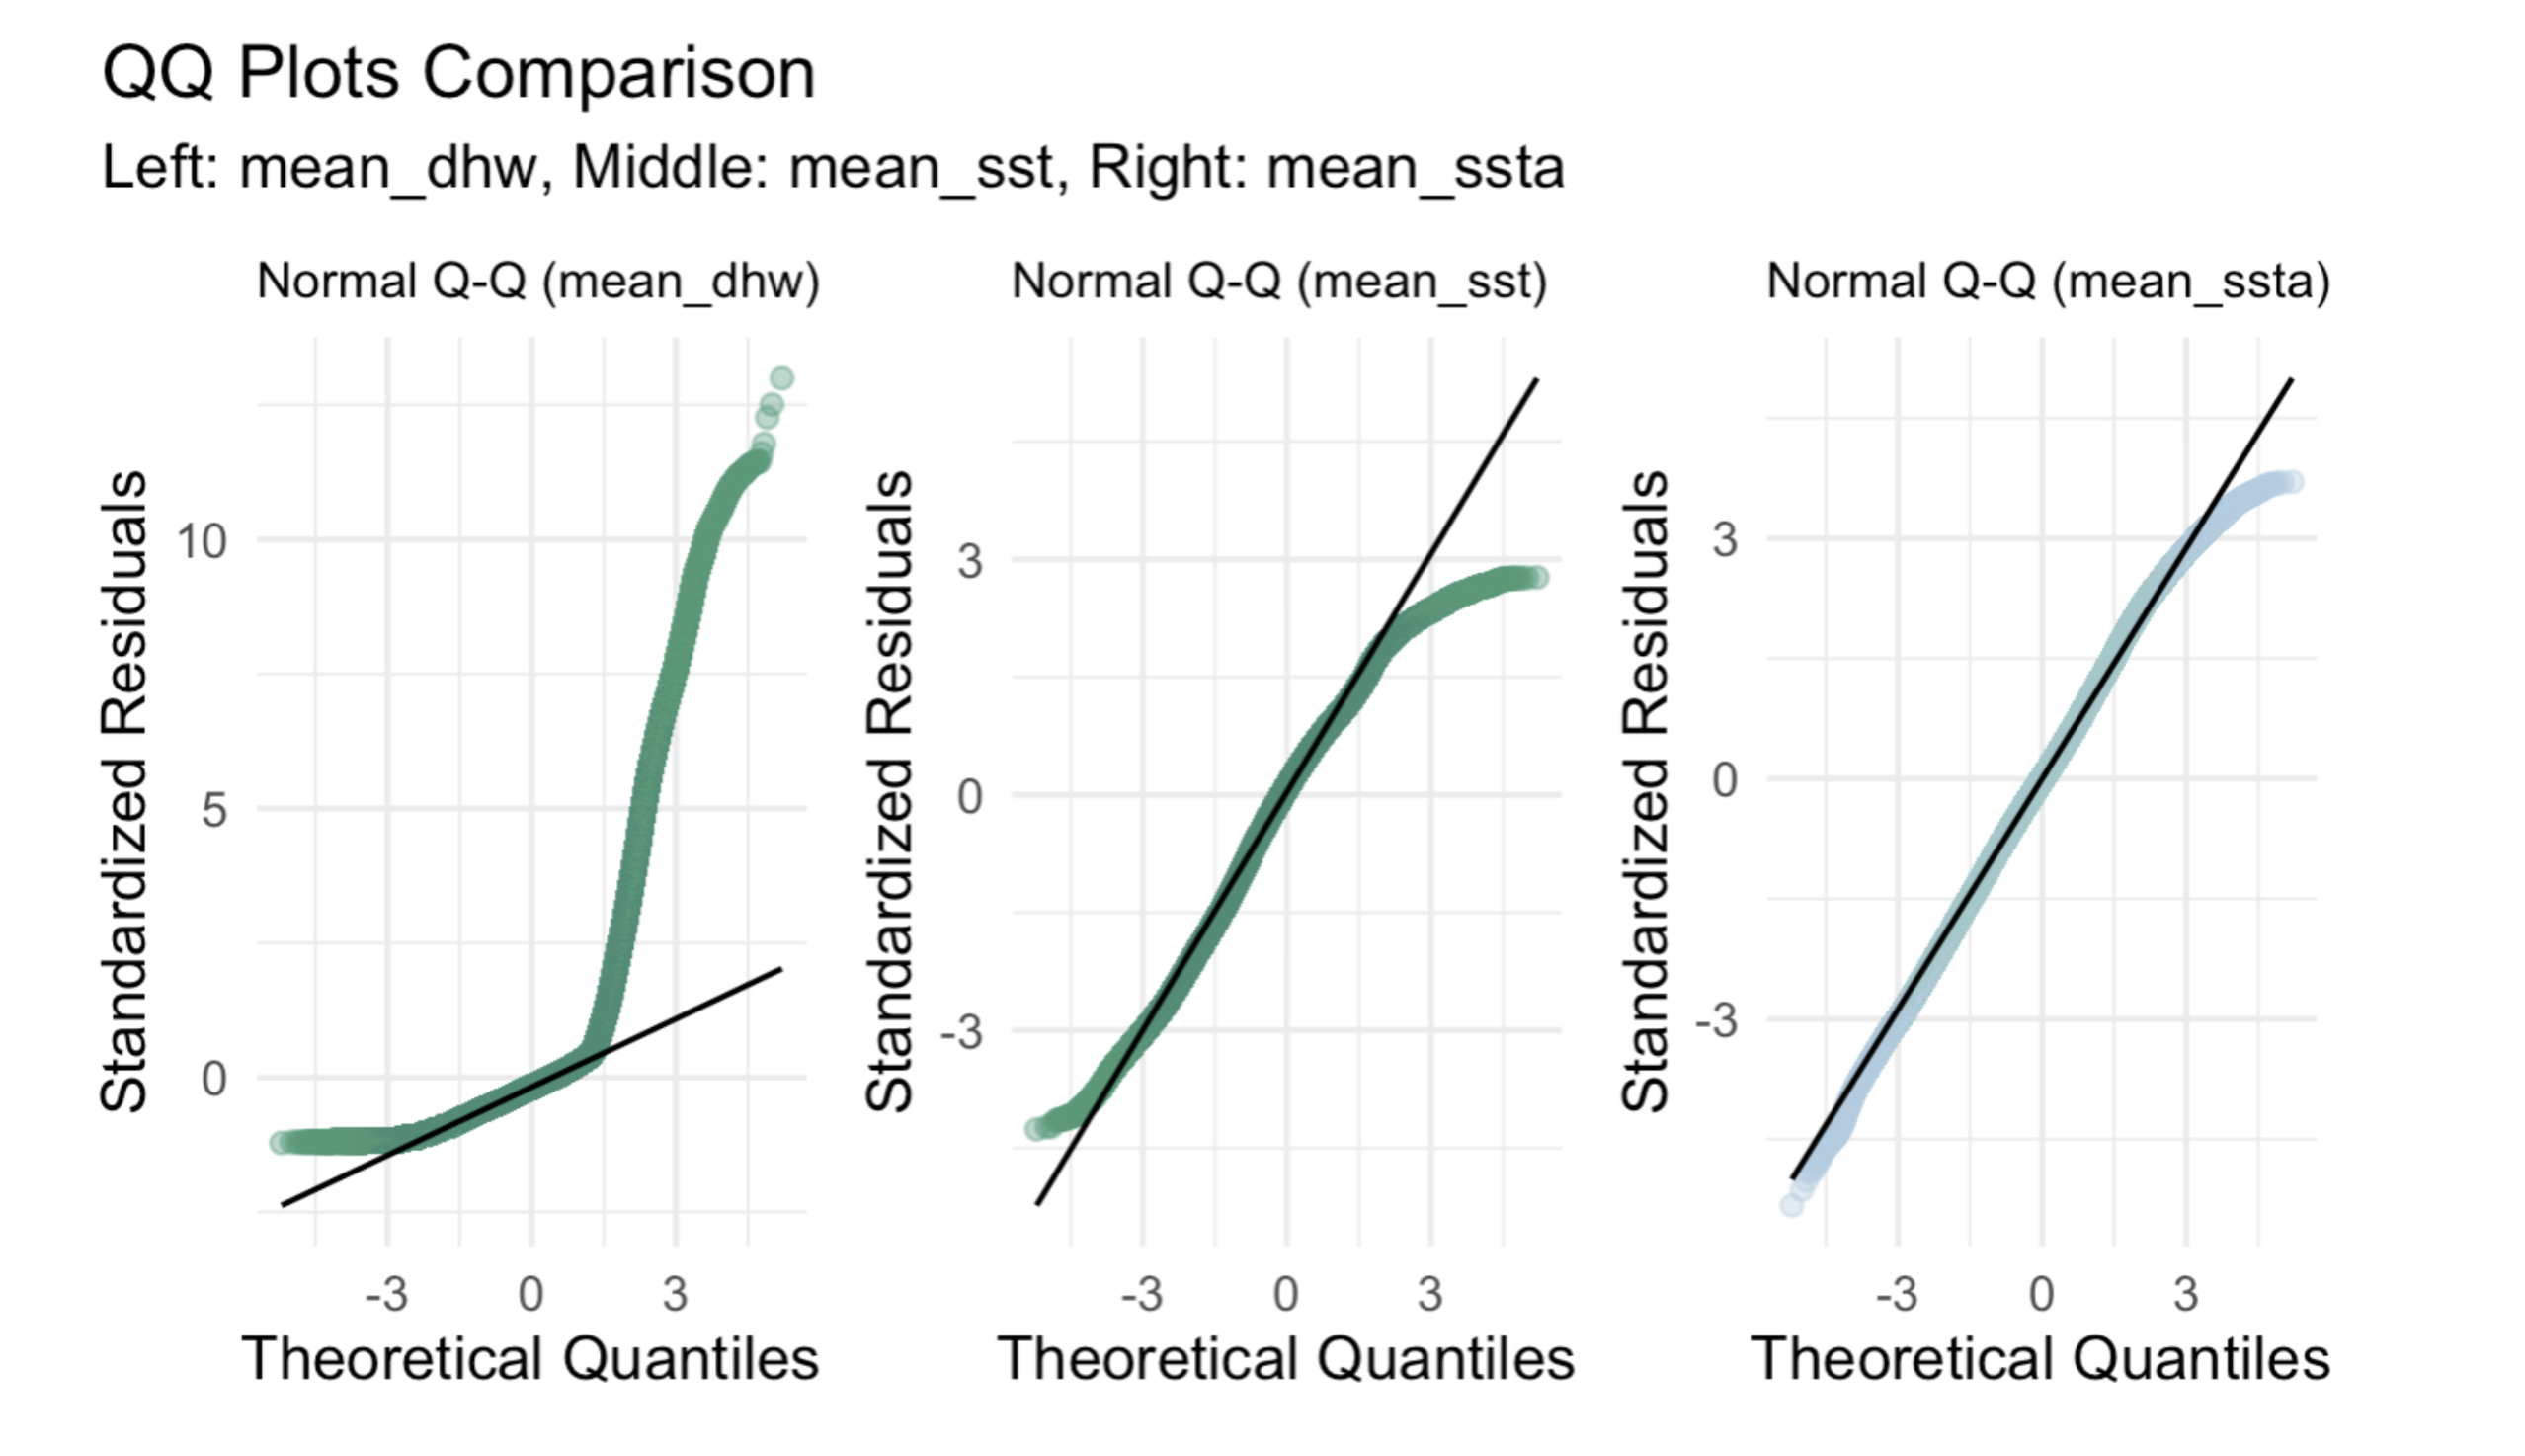
\includegraphics[width=0.5\textwidth]{report_images/lr_qqplots.png}
\end{center}

\begin{center}
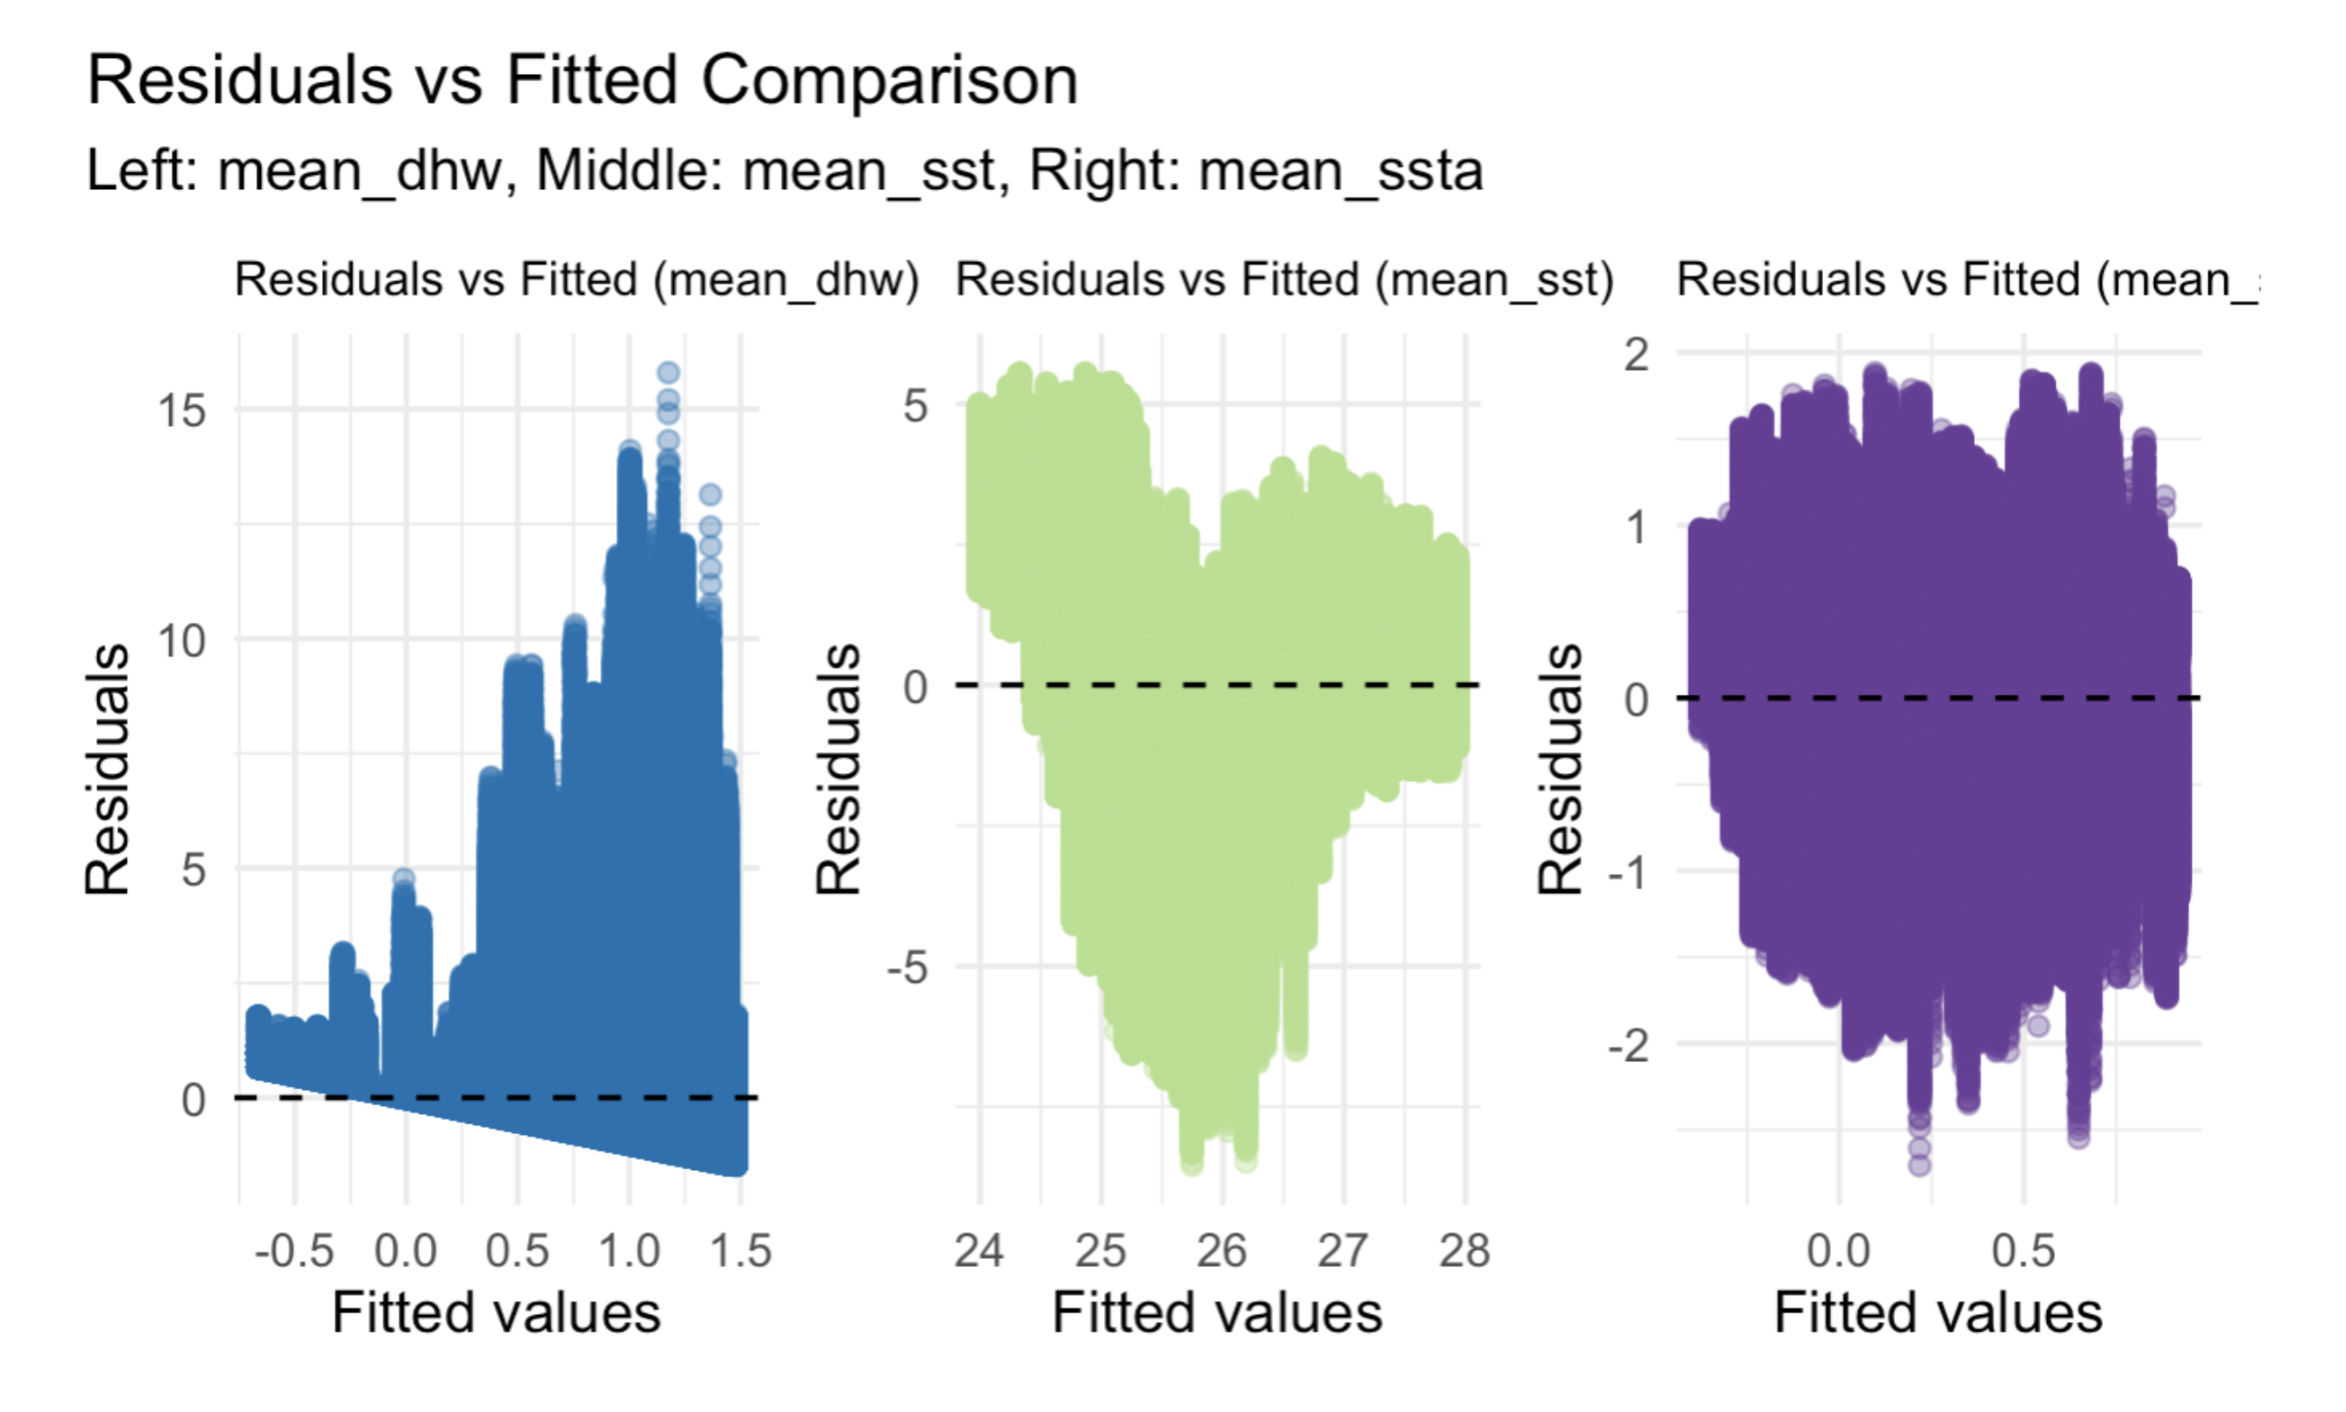
\includegraphics[width=0.5\textwidth]{report_images/lr_resplot.png}
\end{center}

\begin{center}
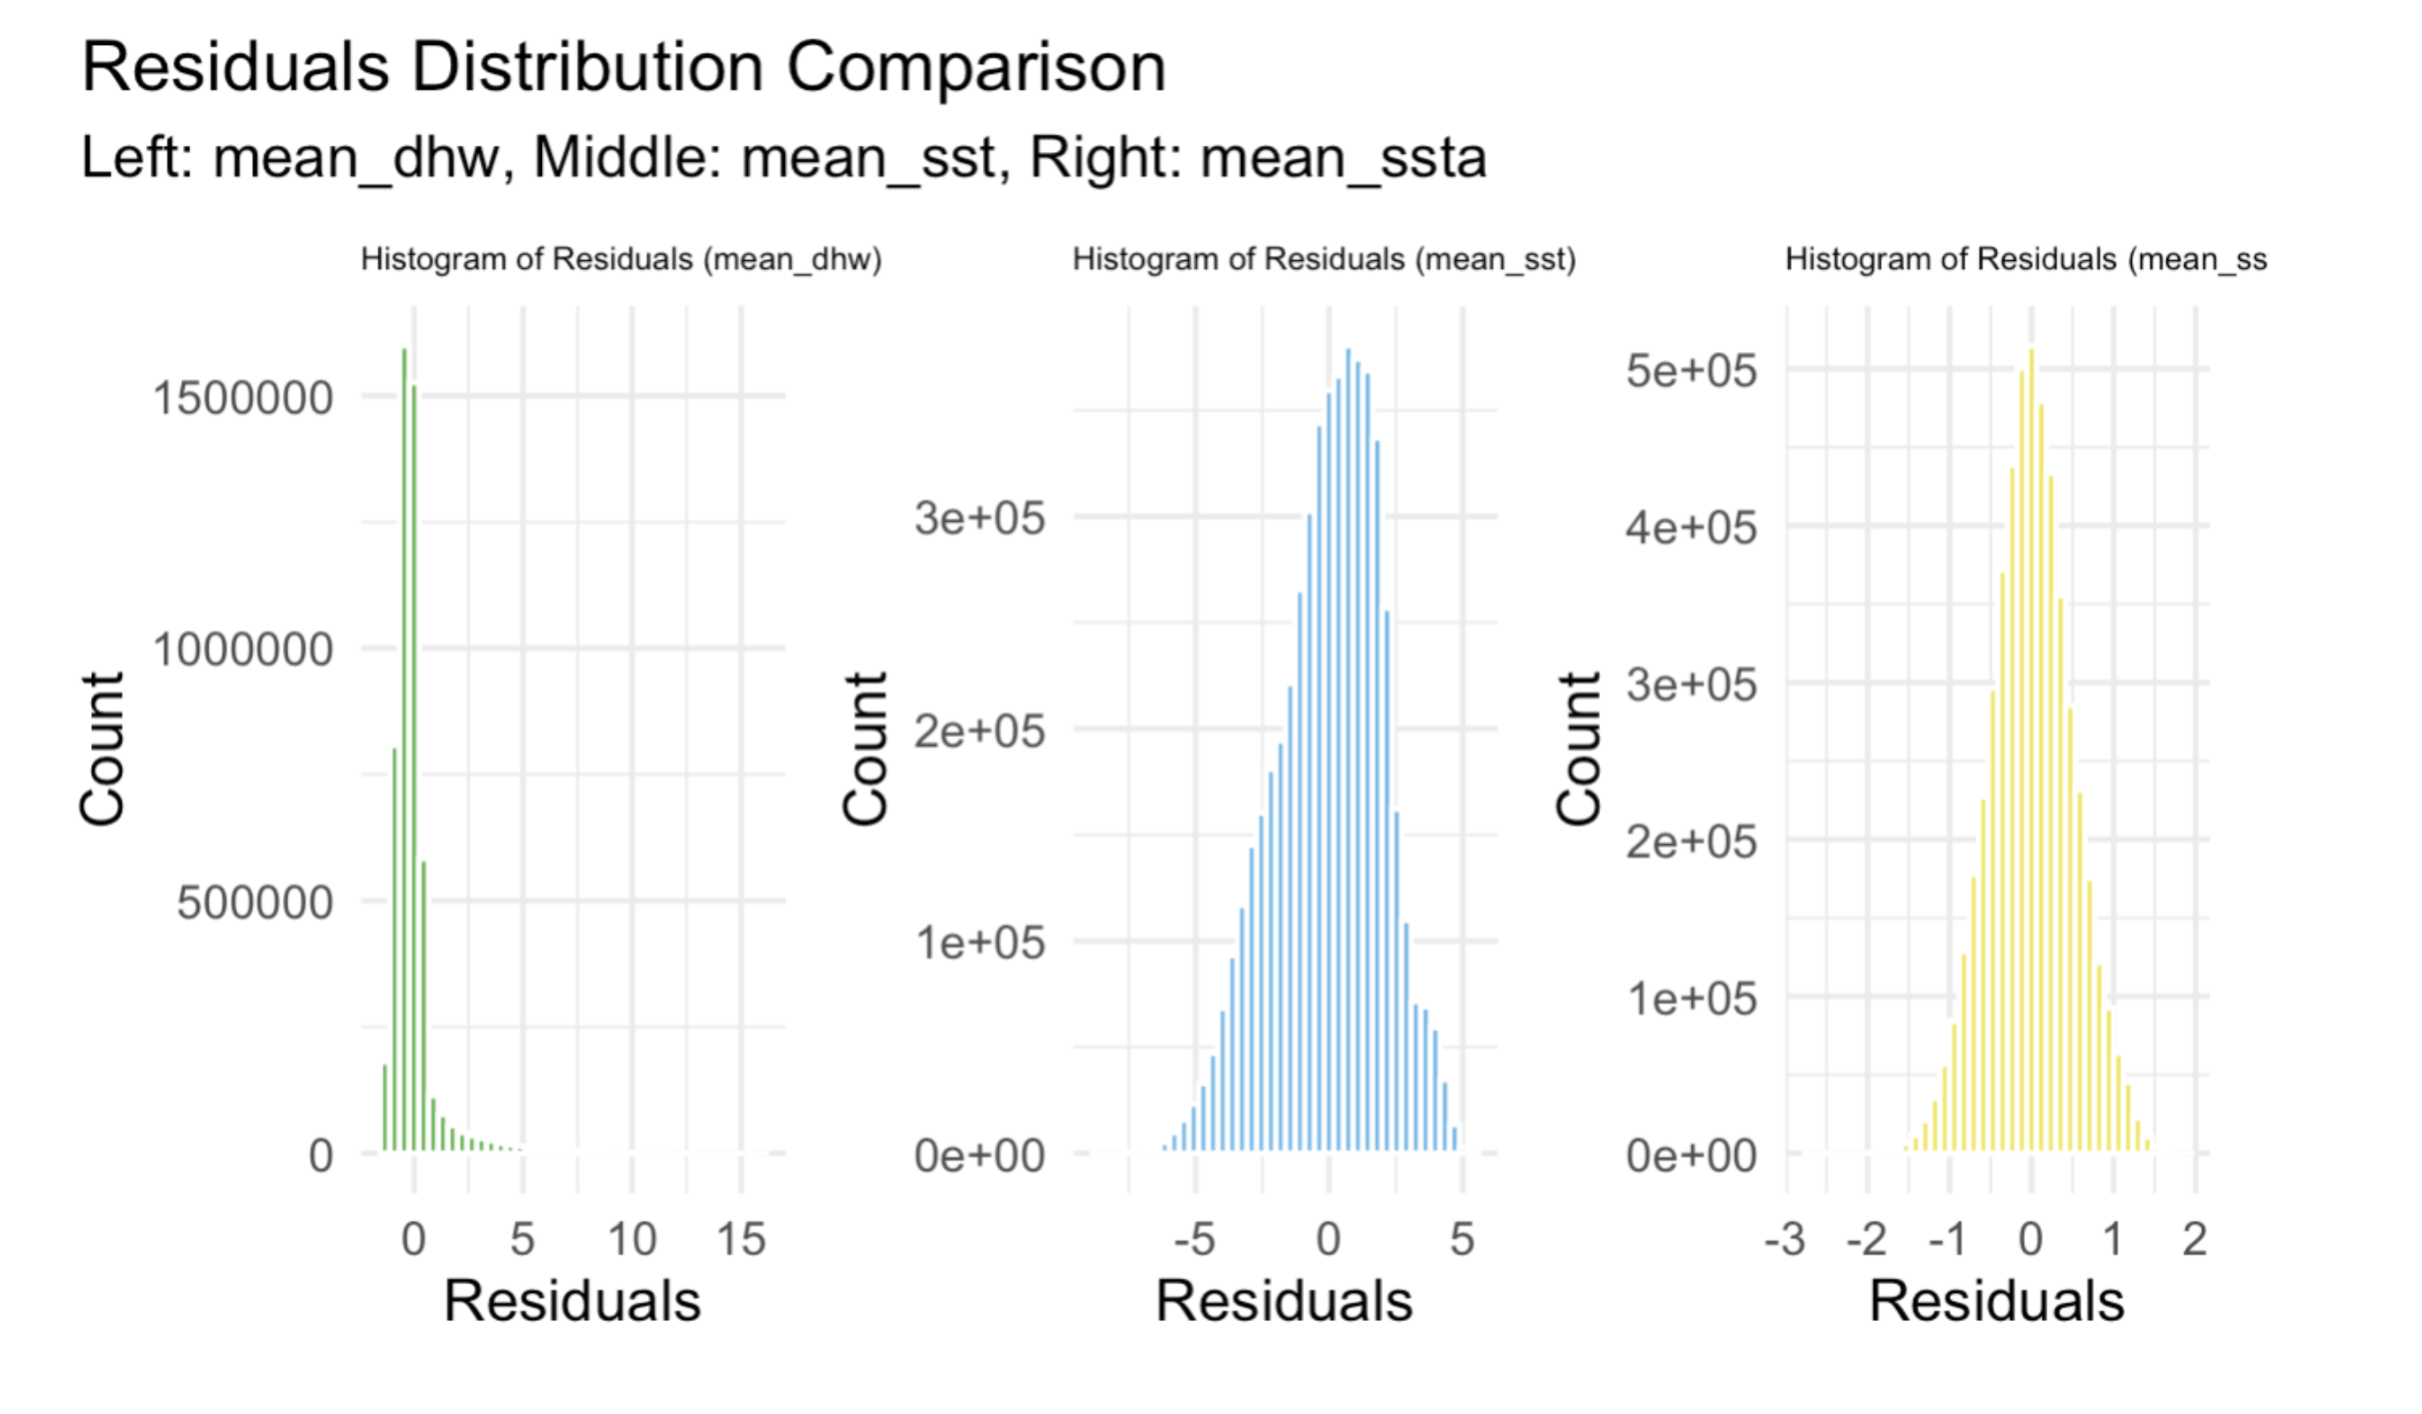
\includegraphics[width=0.5\textwidth]{report_images/lr_reshist.png}
\end{center}

\subsection{Appendix B: Linear Regression Predicted vs
Actual}\label{appendix-b-linear-regression-predicted-vs-actual}

\begin{center}
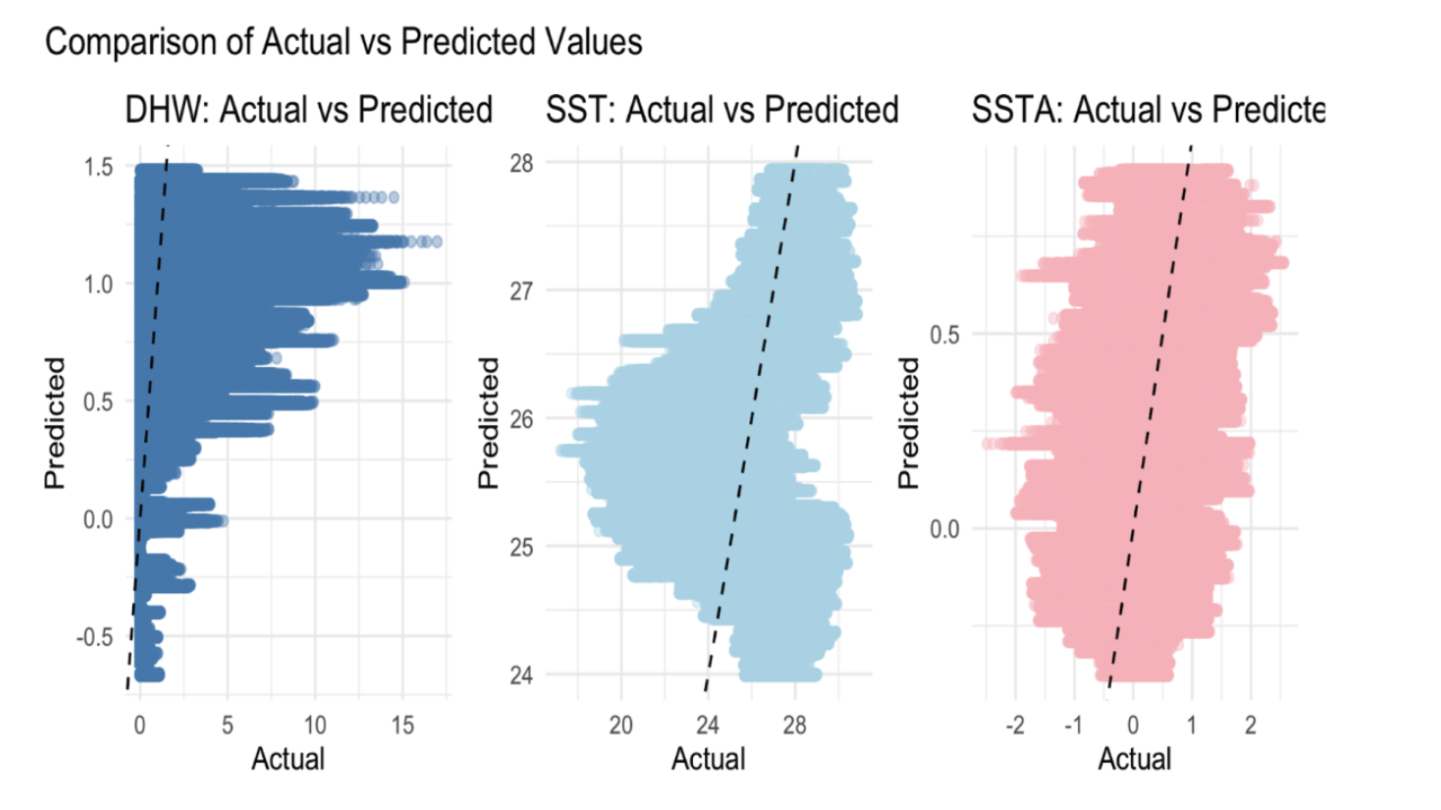
\includegraphics[width=0.5\textwidth]{report_images/lr_graph.png}
\end{center}

\subsection{Appendix C: Mixed Effects Model
Plots}\label{appendix-c-mixed-effects-model-plots}

\begin{center}
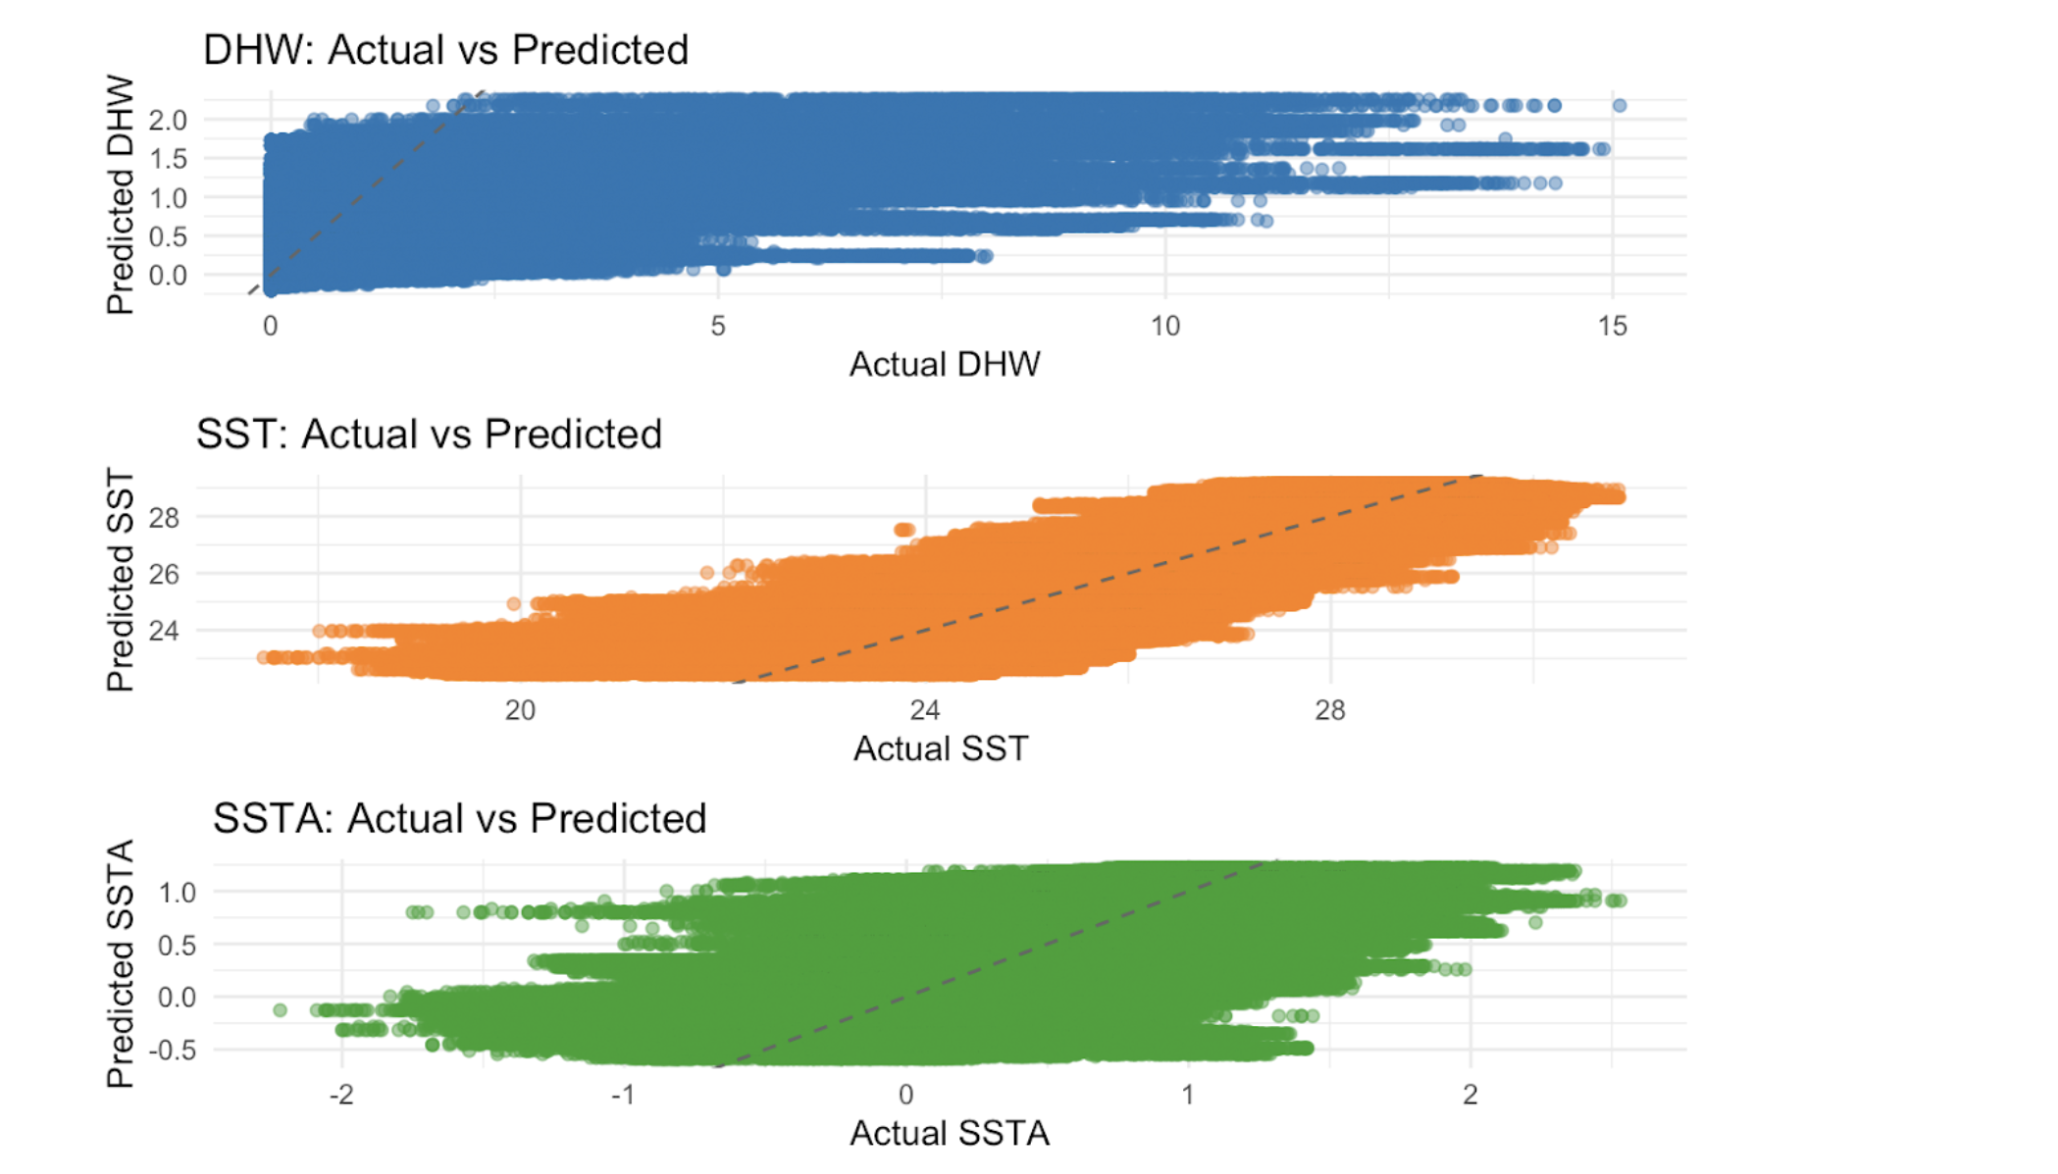
\includegraphics[width=0.5\textwidth]{report_images/mem_plot.png}
\end{center}

\subsection{Appendix D: Random Forest Model
Plots}\label{appendix-d-random-forest-model-plots}

\begin{center}
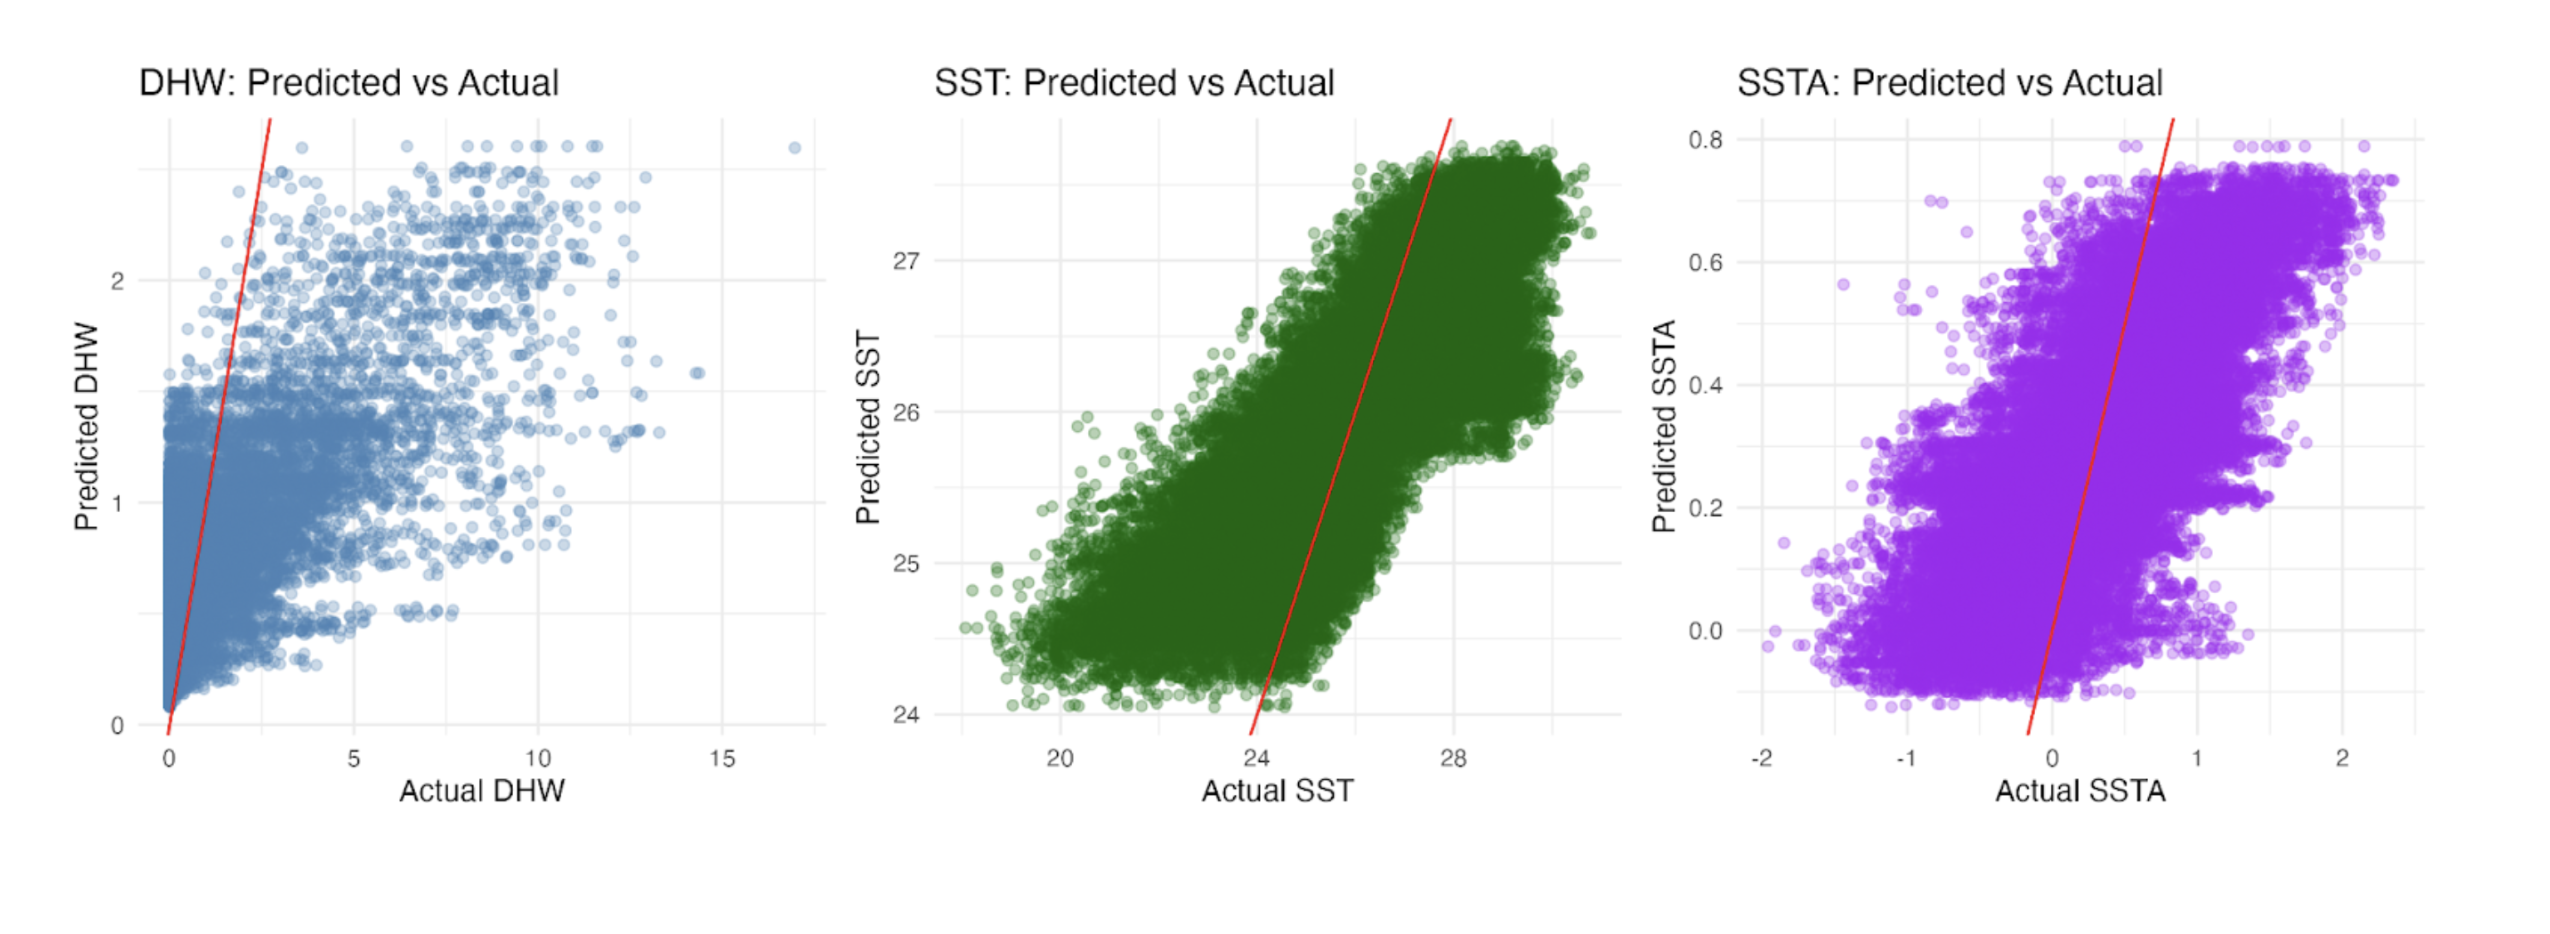
\includegraphics[width=0.5\textwidth]{report_images/rf_predicted_vs_actual.png}
\end{center}

\begin{center}
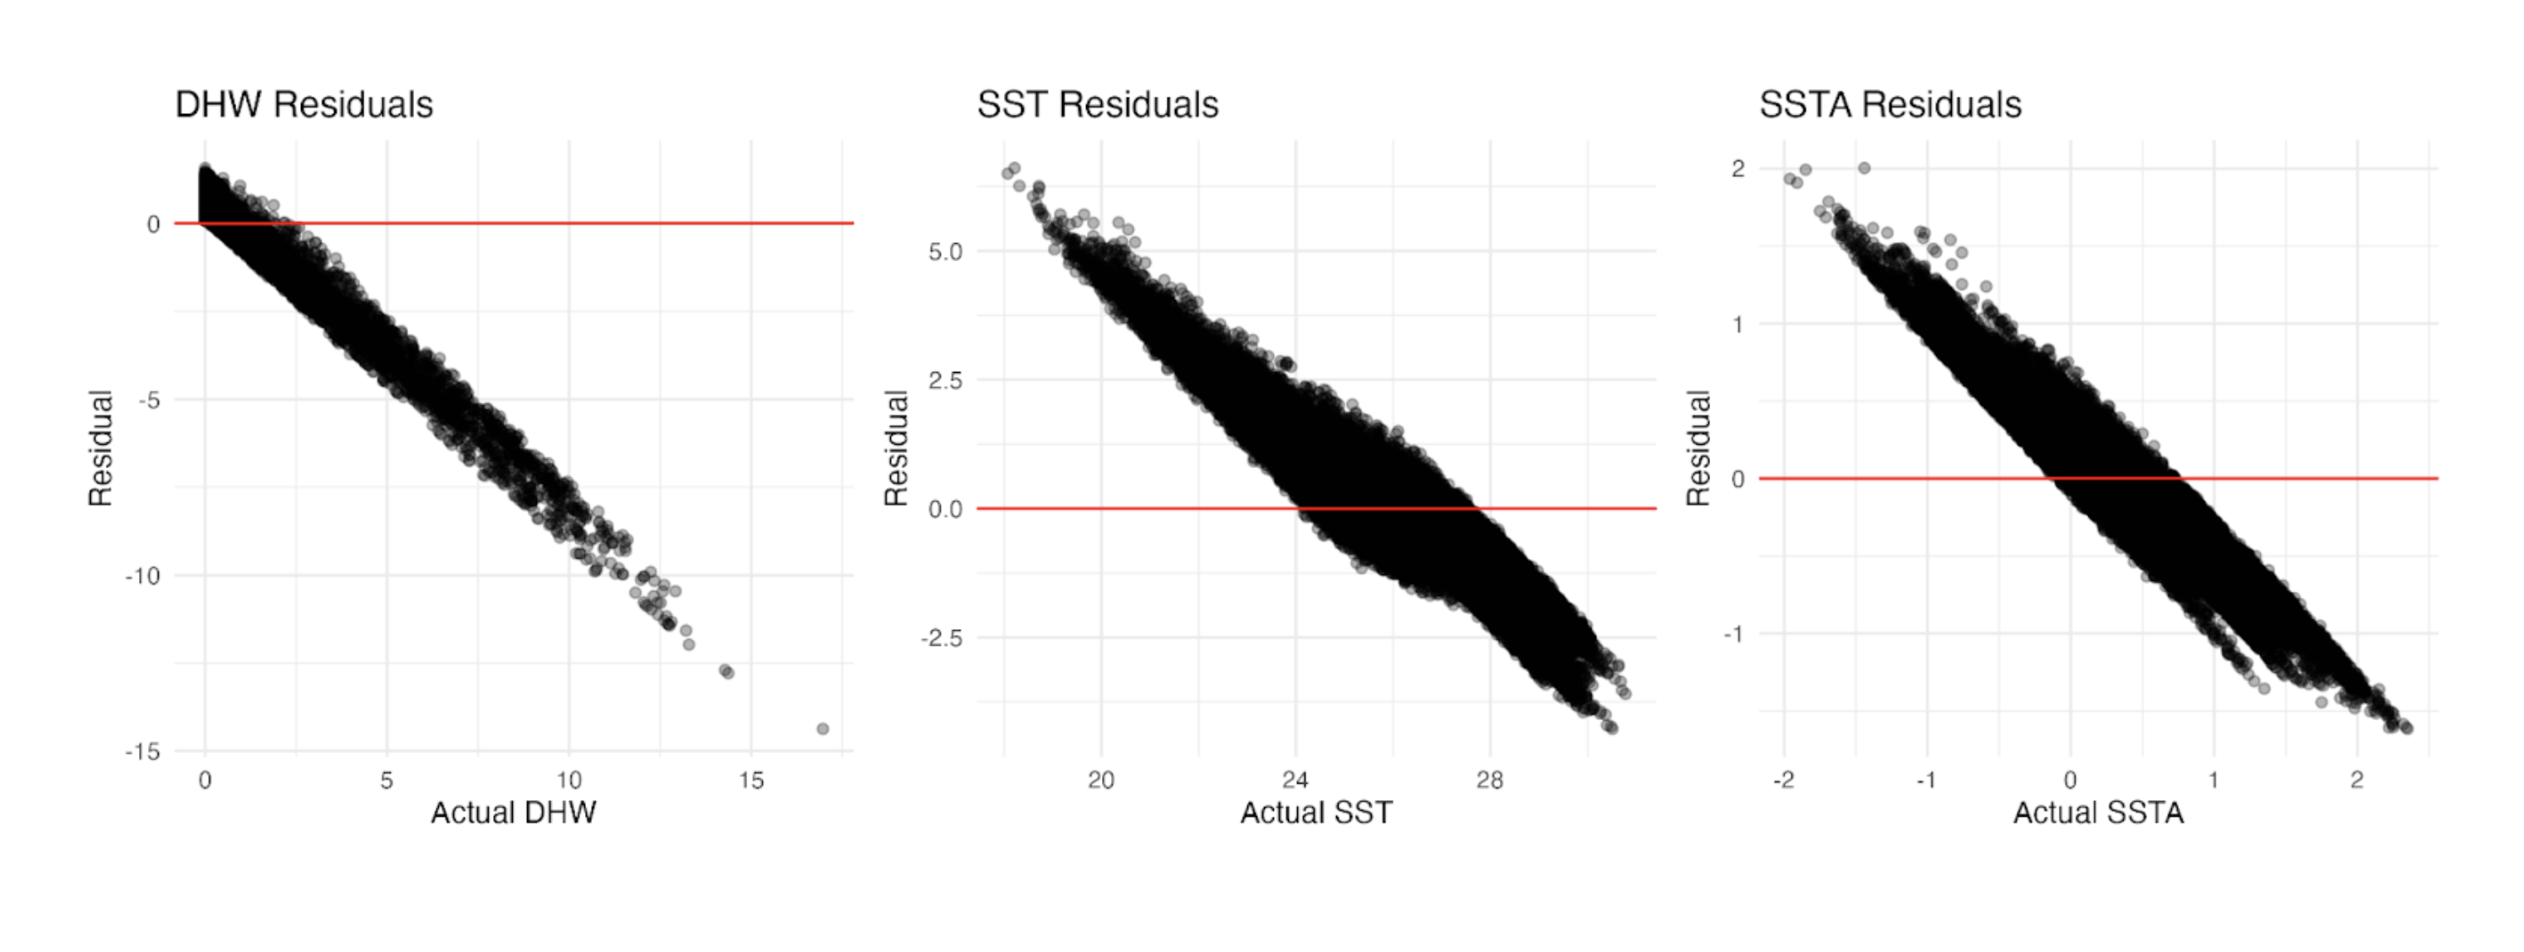
\includegraphics[width=0.5\textwidth]{report_images/rf_residuals.png}
\end{center}

\subsection{Appendix E: Global GAM Model
Summaries}\label{appendix-e-global-gam-model-summaries}

\begin{ShadedResult}
\begin{verbatim}


Table: Smooth Terms for GAM (DHW)

|    edf|       F| p.value|term                   |
|------:|-------:|-------:|:----------------------|
|  6.867|  36.004|   0.000|s(soi_anomaly)         |
|  8.905|  66.803|   0.000|s(year)                |
|  8.177| 161.333|   0.000|s(month)               |
|  1.218|   0.733|   0.344|ti(soi_anomaly):shelfI |
|  1.001|   1.331|   0.249|ti(soi_anomaly):shelfM |
|  1.000|   1.349|   0.246|ti(soi_anomaly):shelfO |
| 15.675| 121.842|   0.000|ti(soi_anomaly,year)   |
| 76.393|  36.669|   0.000|ti(soi_anomaly,month)  |

\end{verbatim}
\end{ShadedResult}

\begin{ShadedResult}
\begin{verbatim}


Table: Smooth Terms for GAM (SST)

|    edf|       F| p.value|term                   |
|------:|-------:|-------:|:----------------------|
|  6.966|  23.320|   0.000|s(soi_anomaly)         |
|  8.957| 120.096|   0.000|s(year)                |
|  9.598| 263.824|   0.000|s(month)               |
|  1.002|   2.561|   0.109|ti(soi_anomaly):shelfI |
|  1.002|   2.353|   0.125|ti(soi_anomaly):shelfM |
|  3.561|  16.385|   0.000|ti(soi_anomaly):shelfO |
| 14.481|  19.844|   0.000|ti(soi_anomaly,year)   |
| 60.950|  14.057|   0.000|ti(soi_anomaly,month)  |

\end{verbatim}
\end{ShadedResult}

\begin{ShadedResult}
\begin{verbatim}


Table: Smooth Terms for GAM (SSTA)

|    edf|       F| p.value|term                   |
|------:|-------:|-------:|:----------------------|
|  7.419| 113.082|   0.000|s(soi_anomaly)         |
|  8.985| 405.180|   0.000|s(year)                |
|  9.775| 139.813|   0.000|s(month)               |
|  2.810|   5.806|   0.000|ti(soi_anomaly):shelfI |
|  1.000|  11.492|   0.001|ti(soi_anomaly):shelfM |
|  1.147|   8.409|   0.002|ti(soi_anomaly):shelfO |
| 15.780|  66.586|   0.000|ti(soi_anomaly,year)   |
| 89.329| 122.515|   0.000|ti(soi_anomaly,month)  |

\end{verbatim}
\end{ShadedResult}

\subsection{Appendix F: Rolling-Validation GAM
Performance}\label{appendix-f-rolling-validation-gam-performance}

\begin{ShadedResult}
\begin{verbatim}


Table: DHW: Yearly GAM Predictions

| year|   RMSE|   MAE|   R2|
|----:|------:|-----:|----:|
| 1987|   0.95|  0.48| 0.76|
| 1988|   2.54|  2.08| 0.08|
| 1989|   0.71|  0.48| 0.02|
| 1990|   2.54|  1.37| 0.20|
| 1991|   6.98|  5.79| 0.01|
| 1992|  64.89| 26.18| 0.01|
| 1993|   2.88|  1.34| 0.00|
| 1994|   2.19|  1.15| 0.08|
| 1995|   1.41|  0.83| 0.05|
| 1996|   7.03|  2.65| 0.12|
| 1997|  14.79|  5.33| 0.01|
| 1998|  32.05|  9.94| 0.23|
| 1999|   4.35|  1.84| 0.00|
| 2000|   0.35|  0.22| 0.05|
| 2001|   0.49|  0.25| 0.07|
| 2002|   1.72|  0.91| 0.04|
| 2003|   0.80|  0.40| 0.14|
| 2004|   1.04|  0.59| 0.49|
| 2005|  30.86|  9.42| 0.05|
| 2006| 111.91| 56.61| 0.11|
| 2007|   0.99|  0.54| 0.08|
| 2008|  64.98| 45.33| 0.03|
| 2009|   1.11|  0.45| 0.02|
| 2010|   1.08|  0.56| 0.02|
| 2011|   5.83|  2.50| 0.04|
| 2012|   0.56|  0.31| 0.23|
| 2013|   0.55|  0.26| 0.33|
| 2014|   0.71|  0.34| 0.02|
| 2015|   1.45|  0.76| 0.01|
| 2016|   2.20|  0.88| 0.30|
| 2017|   2.59|  1.28| 0.61|
| 2018|   0.51|  0.26| 0.04|
| 2019|   0.74|  0.40| 0.06|
| 2020|   2.84|  1.48| 0.61|
| 2021|   1.55|  0.71| 0.09|
| 2022|   5.27|  2.65| 0.01|
| 2023|   0.75|  0.38| 0.24|
| 2024|   2.96|  1.60| 0.78|

\end{verbatim}
\end{ShadedResult}

\begin{ShadedResult}
\begin{verbatim}


Table: SST: Yearly GAM Predictions

| year|        RMSE|        MAE|   R2|
|----:|-----------:|----------:|----:|
| 1987|        0.96|       0.76| 0.83|
| 1988|        1.26|       1.00| 0.64|
| 1989|        1.38|       1.11| 0.70|
| 1990|       10.03|       4.15| 0.05|
| 1991|       66.58|      41.85| 0.14|
| 1992|      494.16|     198.28| 0.08|
| 1993|        1.63|       1.26| 0.39|
| 1994|        4.78|       3.01| 0.00|
| 1995|        3.10|       2.13| 0.13|
| 1996|      241.64|      82.90| 0.01|
| 1997| 12040115.96| 3779527.05| 0.16|
| 1998|    22869.93|   10983.40| 0.17|
| 1999|      551.55|     213.53| 0.00|
| 2000|       29.20|       9.48| 0.04|
| 2001|    13827.85|    4014.78| 0.01|
| 2002|        2.01|       1.50| 0.29|
| 2003|        1.11|       0.89| 0.71|
| 2004|        1.25|       1.05| 0.70|
| 2005|        9.04|       3.36| 0.26|
| 2006|    32292.07|   17444.60| 0.01|
| 2007|     1826.50|    1128.50| 0.01|
| 2008|     8019.42|    4174.02| 0.01|
| 2009|        1.23|       1.00| 0.70|
| 2010|      264.24|      81.55| 0.11|
| 2011|        3.10|       1.86| 0.50|
| 2012|        1.19|       0.95| 0.74|
| 2013|        1.20|       0.97| 0.73|
| 2014|        1.48|       1.07| 0.59|
| 2015|        3.95|       1.92| 0.03|
| 2016|        1.50|       1.22| 0.67|
| 2017|        1.19|       0.99| 0.77|
| 2018|        1.10|       0.90| 0.78|
| 2019|        0.98|       0.79| 0.79|
| 2020|        1.14|       0.95| 0.79|
| 2021|        1.31|       1.05| 0.67|
| 2022|        7.77|       3.62| 0.13|
| 2023|        1.32|       1.05| 0.70|
| 2024|        1.20|       0.99| 0.79|

\end{verbatim}
\end{ShadedResult}

\begin{ShadedResult}
\begin{verbatim}


Table: SSTA: Yearly GAM Predictions

| year|     RMSE|     MAE|   R2|
|----:|--------:|-------:|----:|
| 1987|     0.21|    0.16| 0.77|
| 1988|     0.62|    0.51| 0.01|
| 1989|     0.81|    0.66| 0.15|
| 1990|     3.38|    1.91| 0.02|
| 1991|    44.18|   25.76| 0.02|
| 1992|   350.31|  142.25| 0.12|
| 1993|  5744.99| 3160.26| 0.03|
| 1994|     3.09|    1.83| 0.00|
| 1995|    15.11|    8.49| 0.13|
| 1996|   488.27|  216.44| 0.00|
| 1997|   662.24|  204.48| 0.07|
| 1998| 15820.48| 6241.22| 0.00|
| 1999|    22.04|    7.25| 0.05|
| 2000|  1151.01|  355.29| 0.07|
| 2001|     5.12|    2.05| 0.00|
| 2002|     1.36|    1.04| 0.15|
| 2003|     0.55|    0.45| 0.00|
| 2004|     0.71|    0.57| 0.07|
| 2005|    12.03|    3.83| 0.03|
| 2006|     0.69|    0.54| 0.17|
| 2007|     0.62|    0.51| 0.00|
| 2008|     0.94|    0.74| 0.01|
| 2009|     0.77|    0.65| 0.00|
| 2010|    36.34|   13.23| 0.03|
| 2011|     4.02|    1.81| 0.19|
| 2012|     0.46|    0.37| 0.02|
| 2013|     0.80|    0.61| 0.00|
| 2014|     1.57|    0.77| 0.02|
| 2015|     3.75|    1.74| 0.34|
| 2016|     1.05|    0.92| 0.00|
| 2017|     0.82|    0.68| 0.00|
| 2018|     0.50|    0.43| 0.01|
| 2019|     0.36|    0.29| 0.22|
| 2020|     0.52|    0.43| 0.32|
| 2021|     0.70|    0.59| 0.00|
| 2022|     7.52|    2.99| 0.00|
| 2023|     0.85|    0.68| 0.10|
| 2024|     0.75|    0.67| 0.04|

\end{verbatim}
\end{ShadedResult}

\subsection{Appendix G: Global GAM `SOI' Smoothed Functions by
`Shelf'}\label{appendix-g-global-gam-soi-smoothed-functions-by-shelf}

\begin{center}
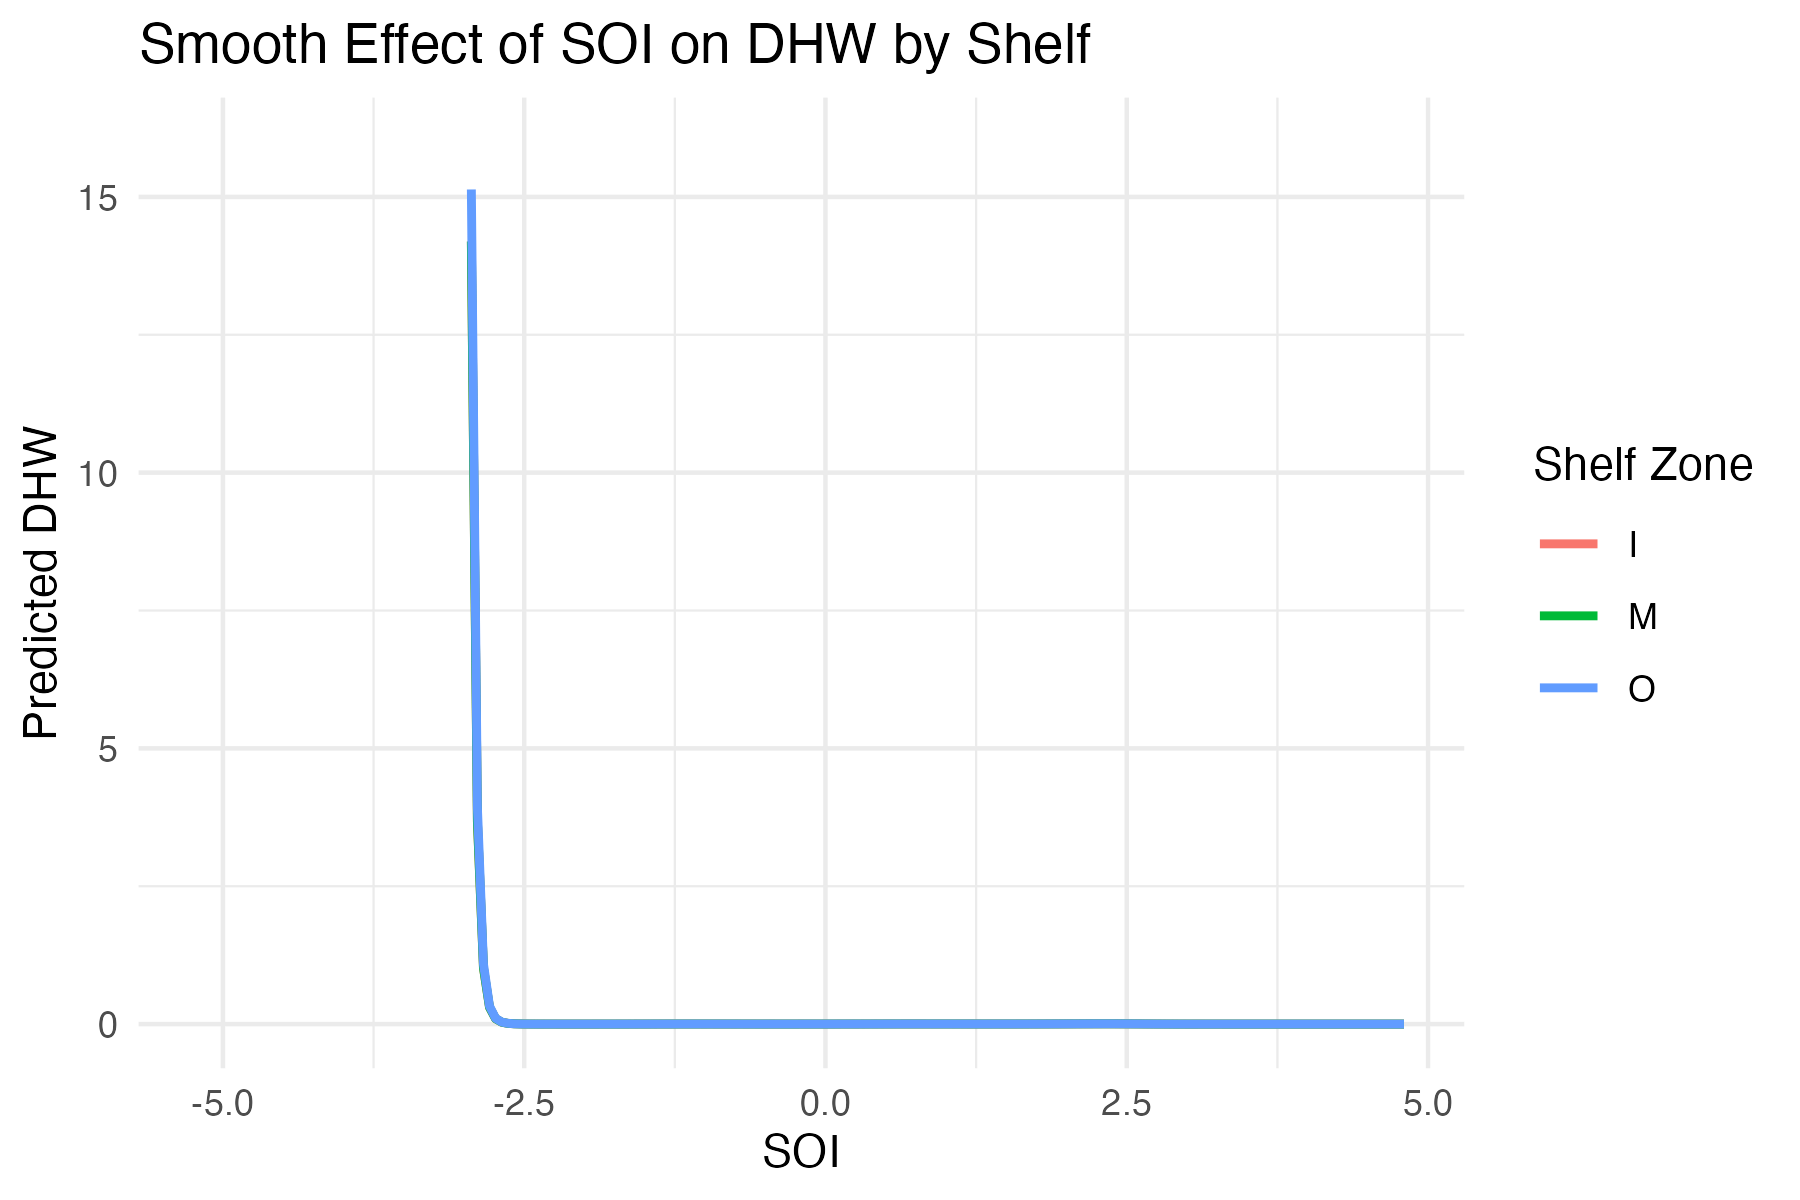
\includegraphics[width=0.5\textwidth]{report_images/soi_shelf_dhw.png}
\end{center}

\begin{center}
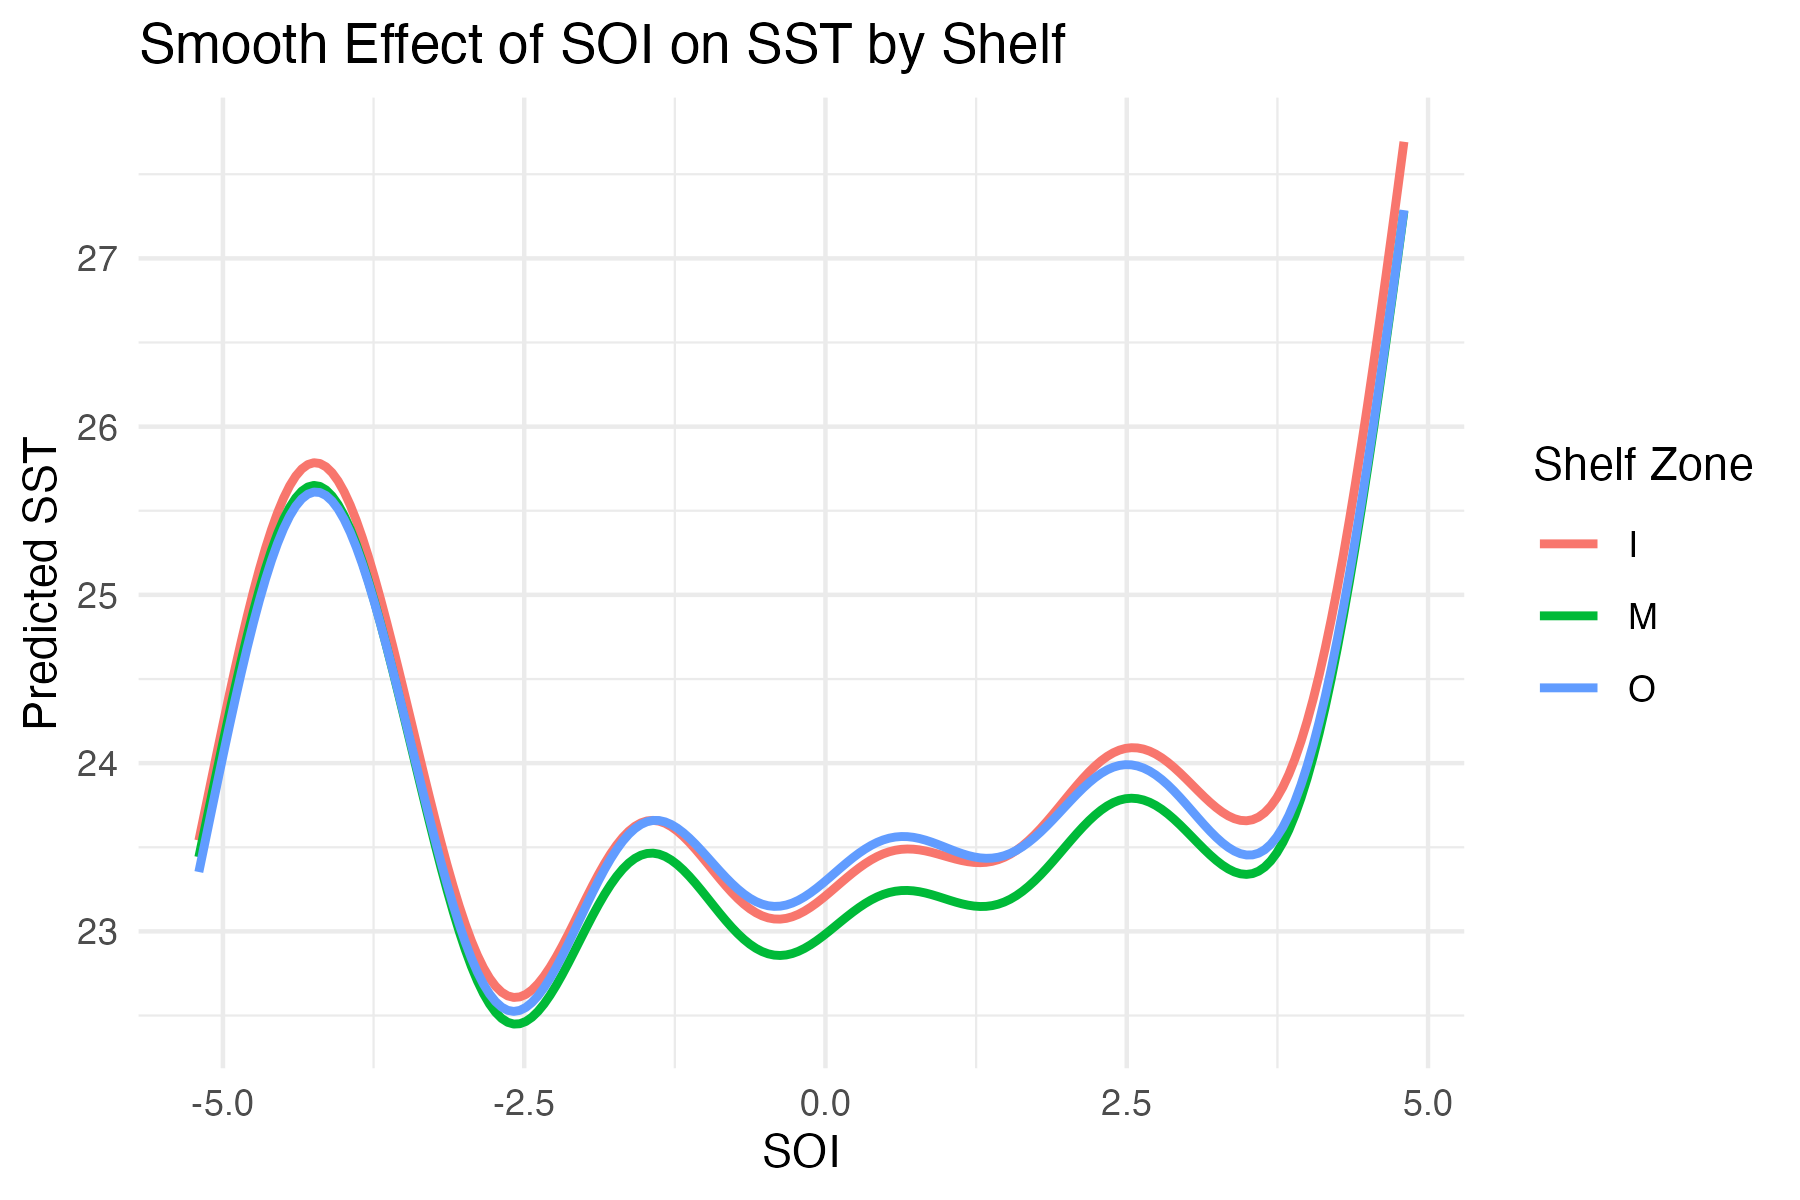
\includegraphics[width=0.5\textwidth]{report_images/soi_shelf_sst.png}
\end{center}

\begin{center}
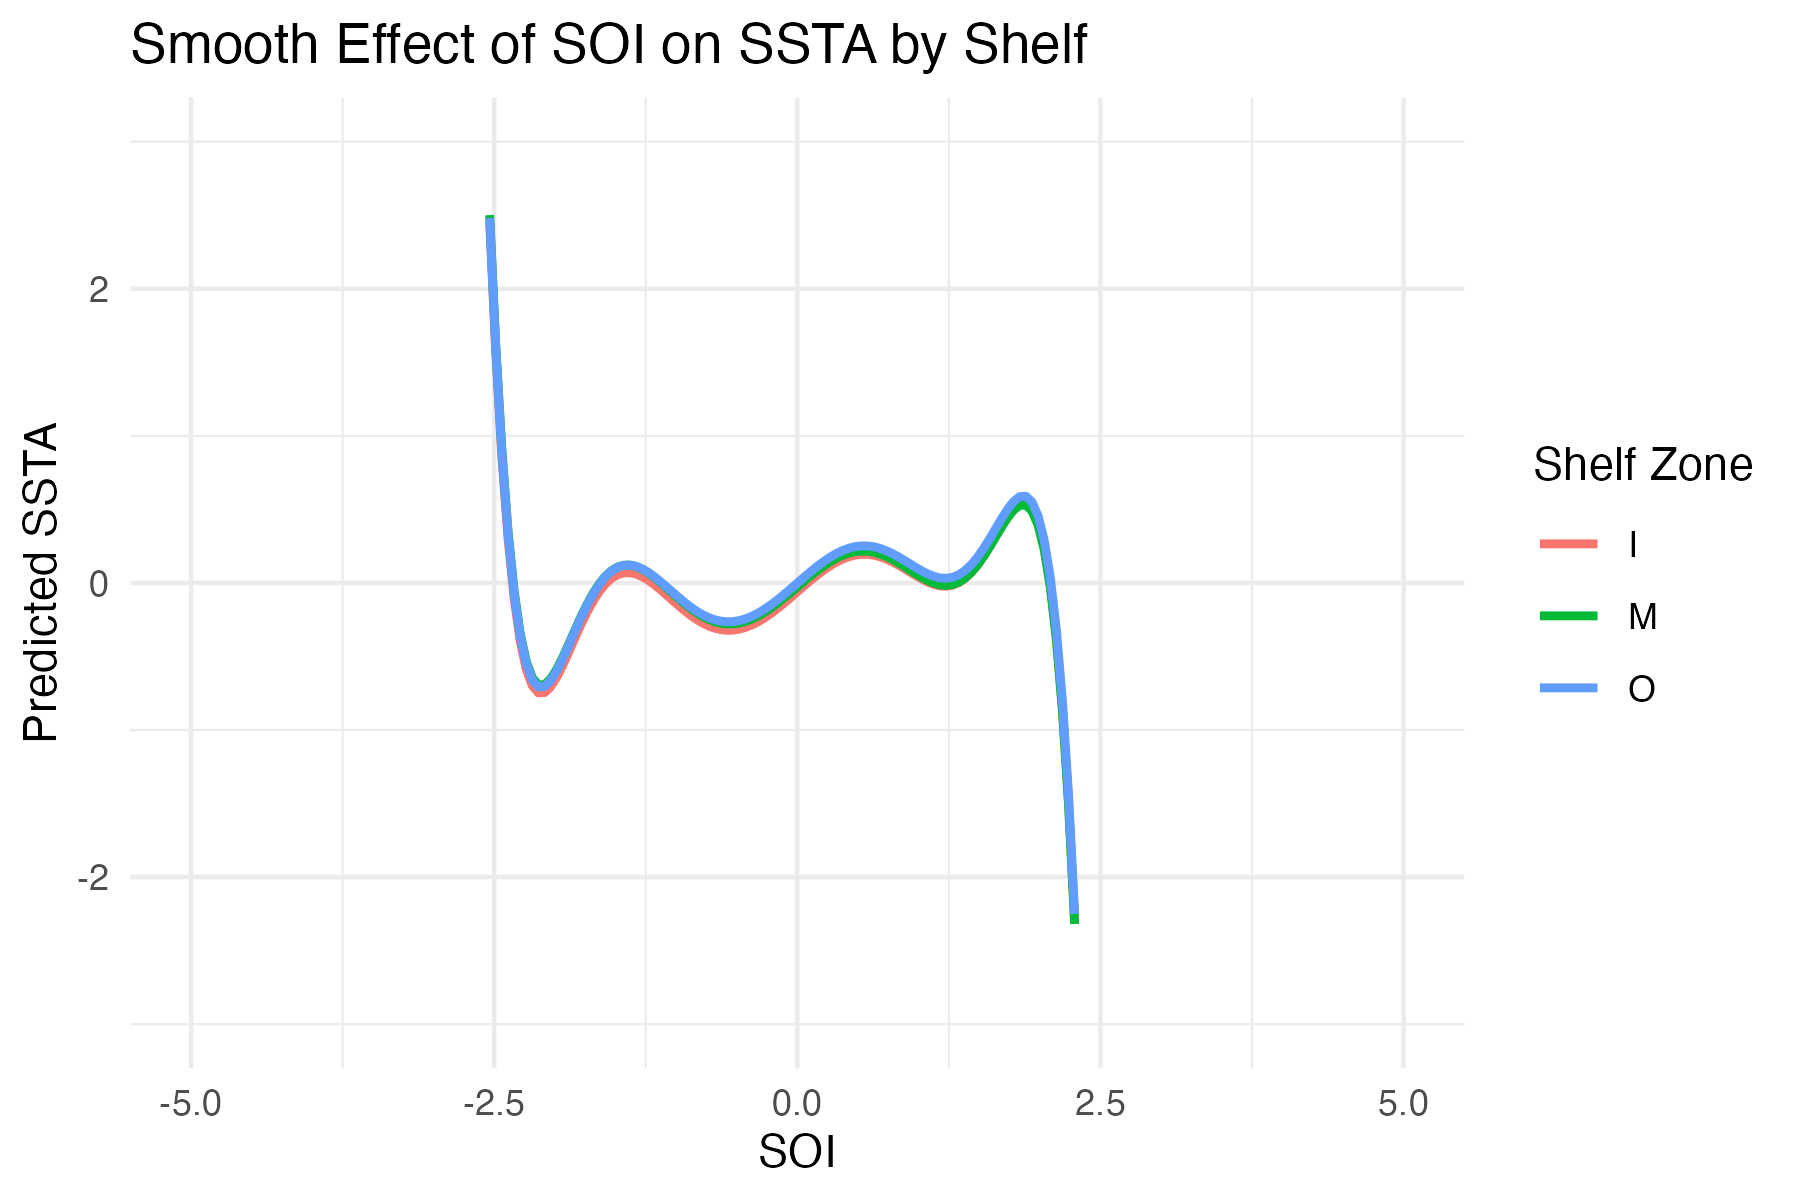
\includegraphics[width=0.5\textwidth]{report_images/soi_shelf_ssta.png}
\end{center}

\subsection{Appendix H: Global GAM `SOI' Smoothed Functions by
`Month'}\label{appendix-h-global-gam-soi-smoothed-functions-by-month}

\begin{center}
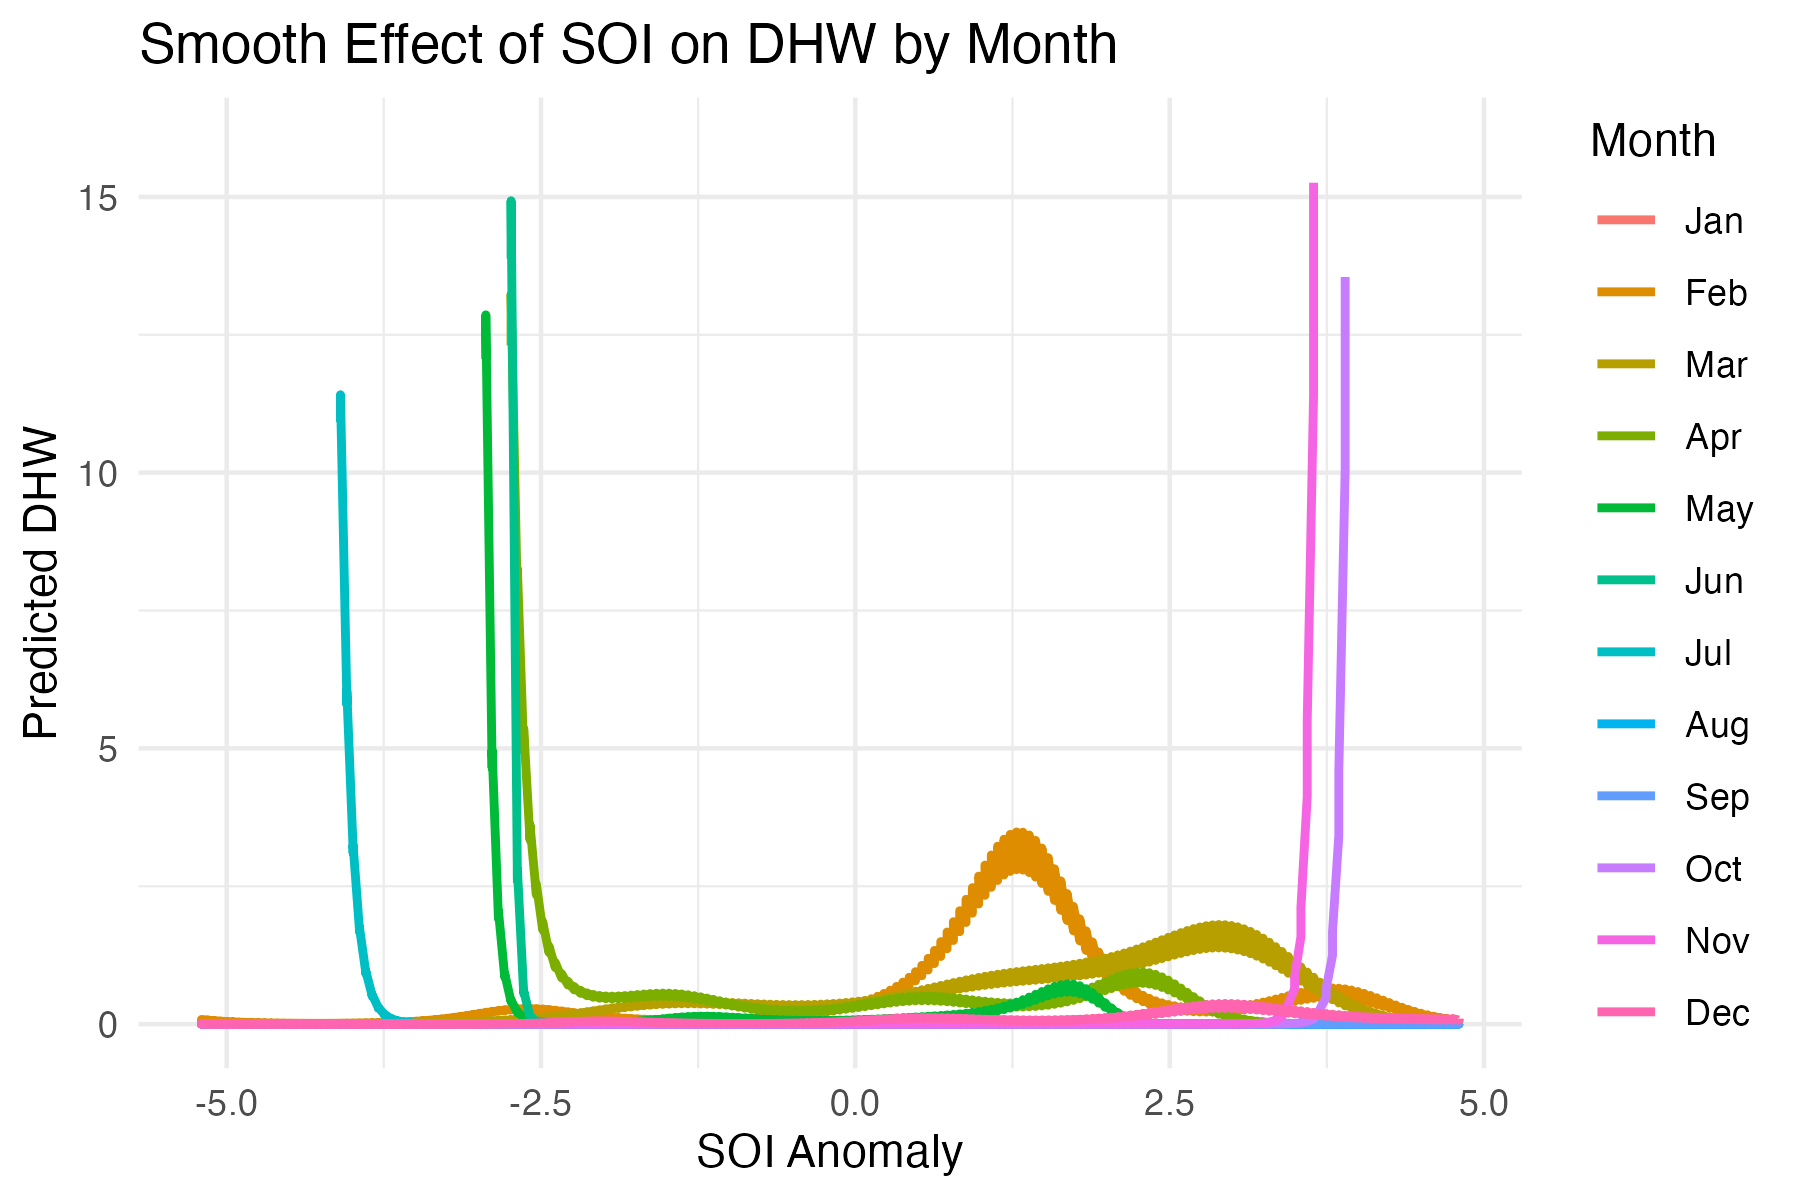
\includegraphics[width=0.5\textwidth]{report_images/soi_month_dhw.png}
\end{center}

\begin{center}
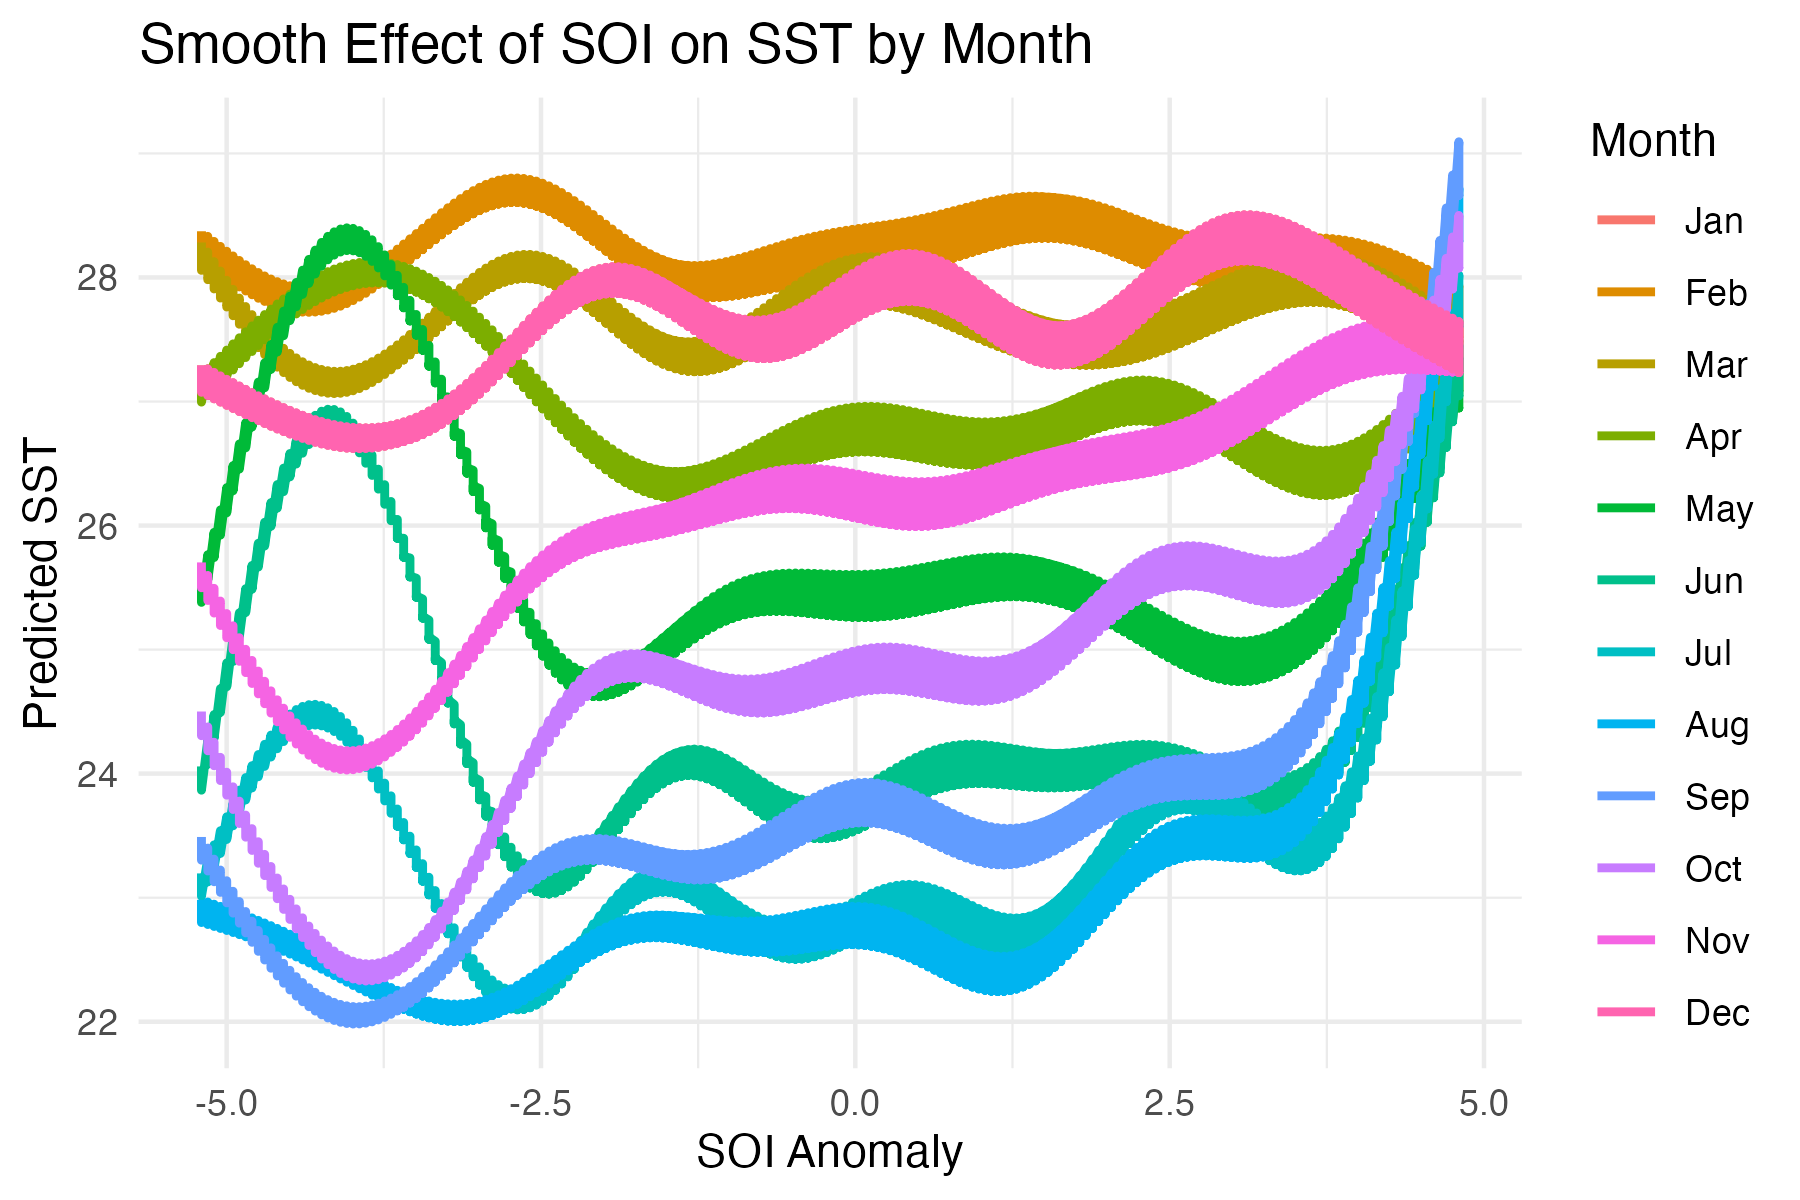
\includegraphics[width=0.5\textwidth]{report_images/soi_month_sst.png}
\end{center}

\begin{center}
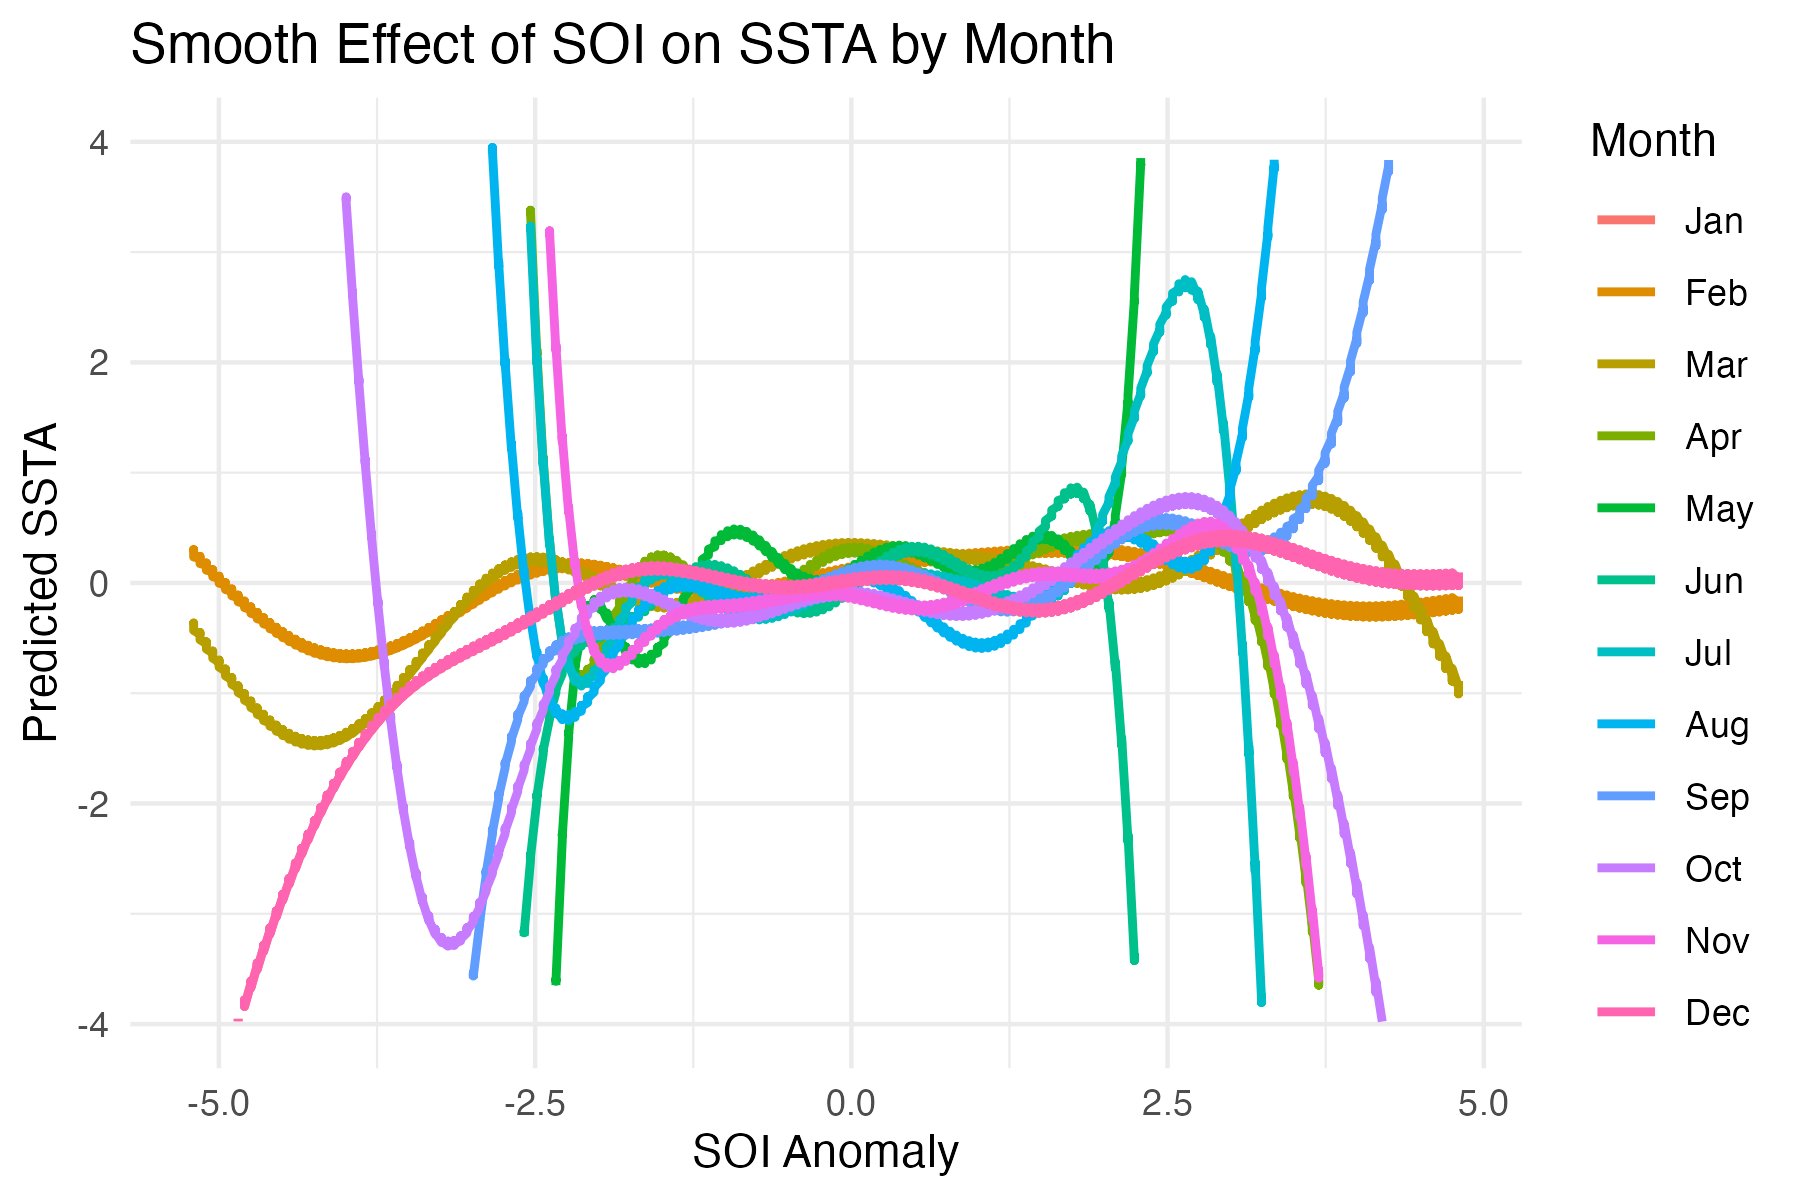
\includegraphics[width=0.5\textwidth]{report_images/soi_month_ssta.png}
\end{center}

\subsection{Appendix I: Shiny
Application}\label{appendix-i-shiny-application}

\begin{center}
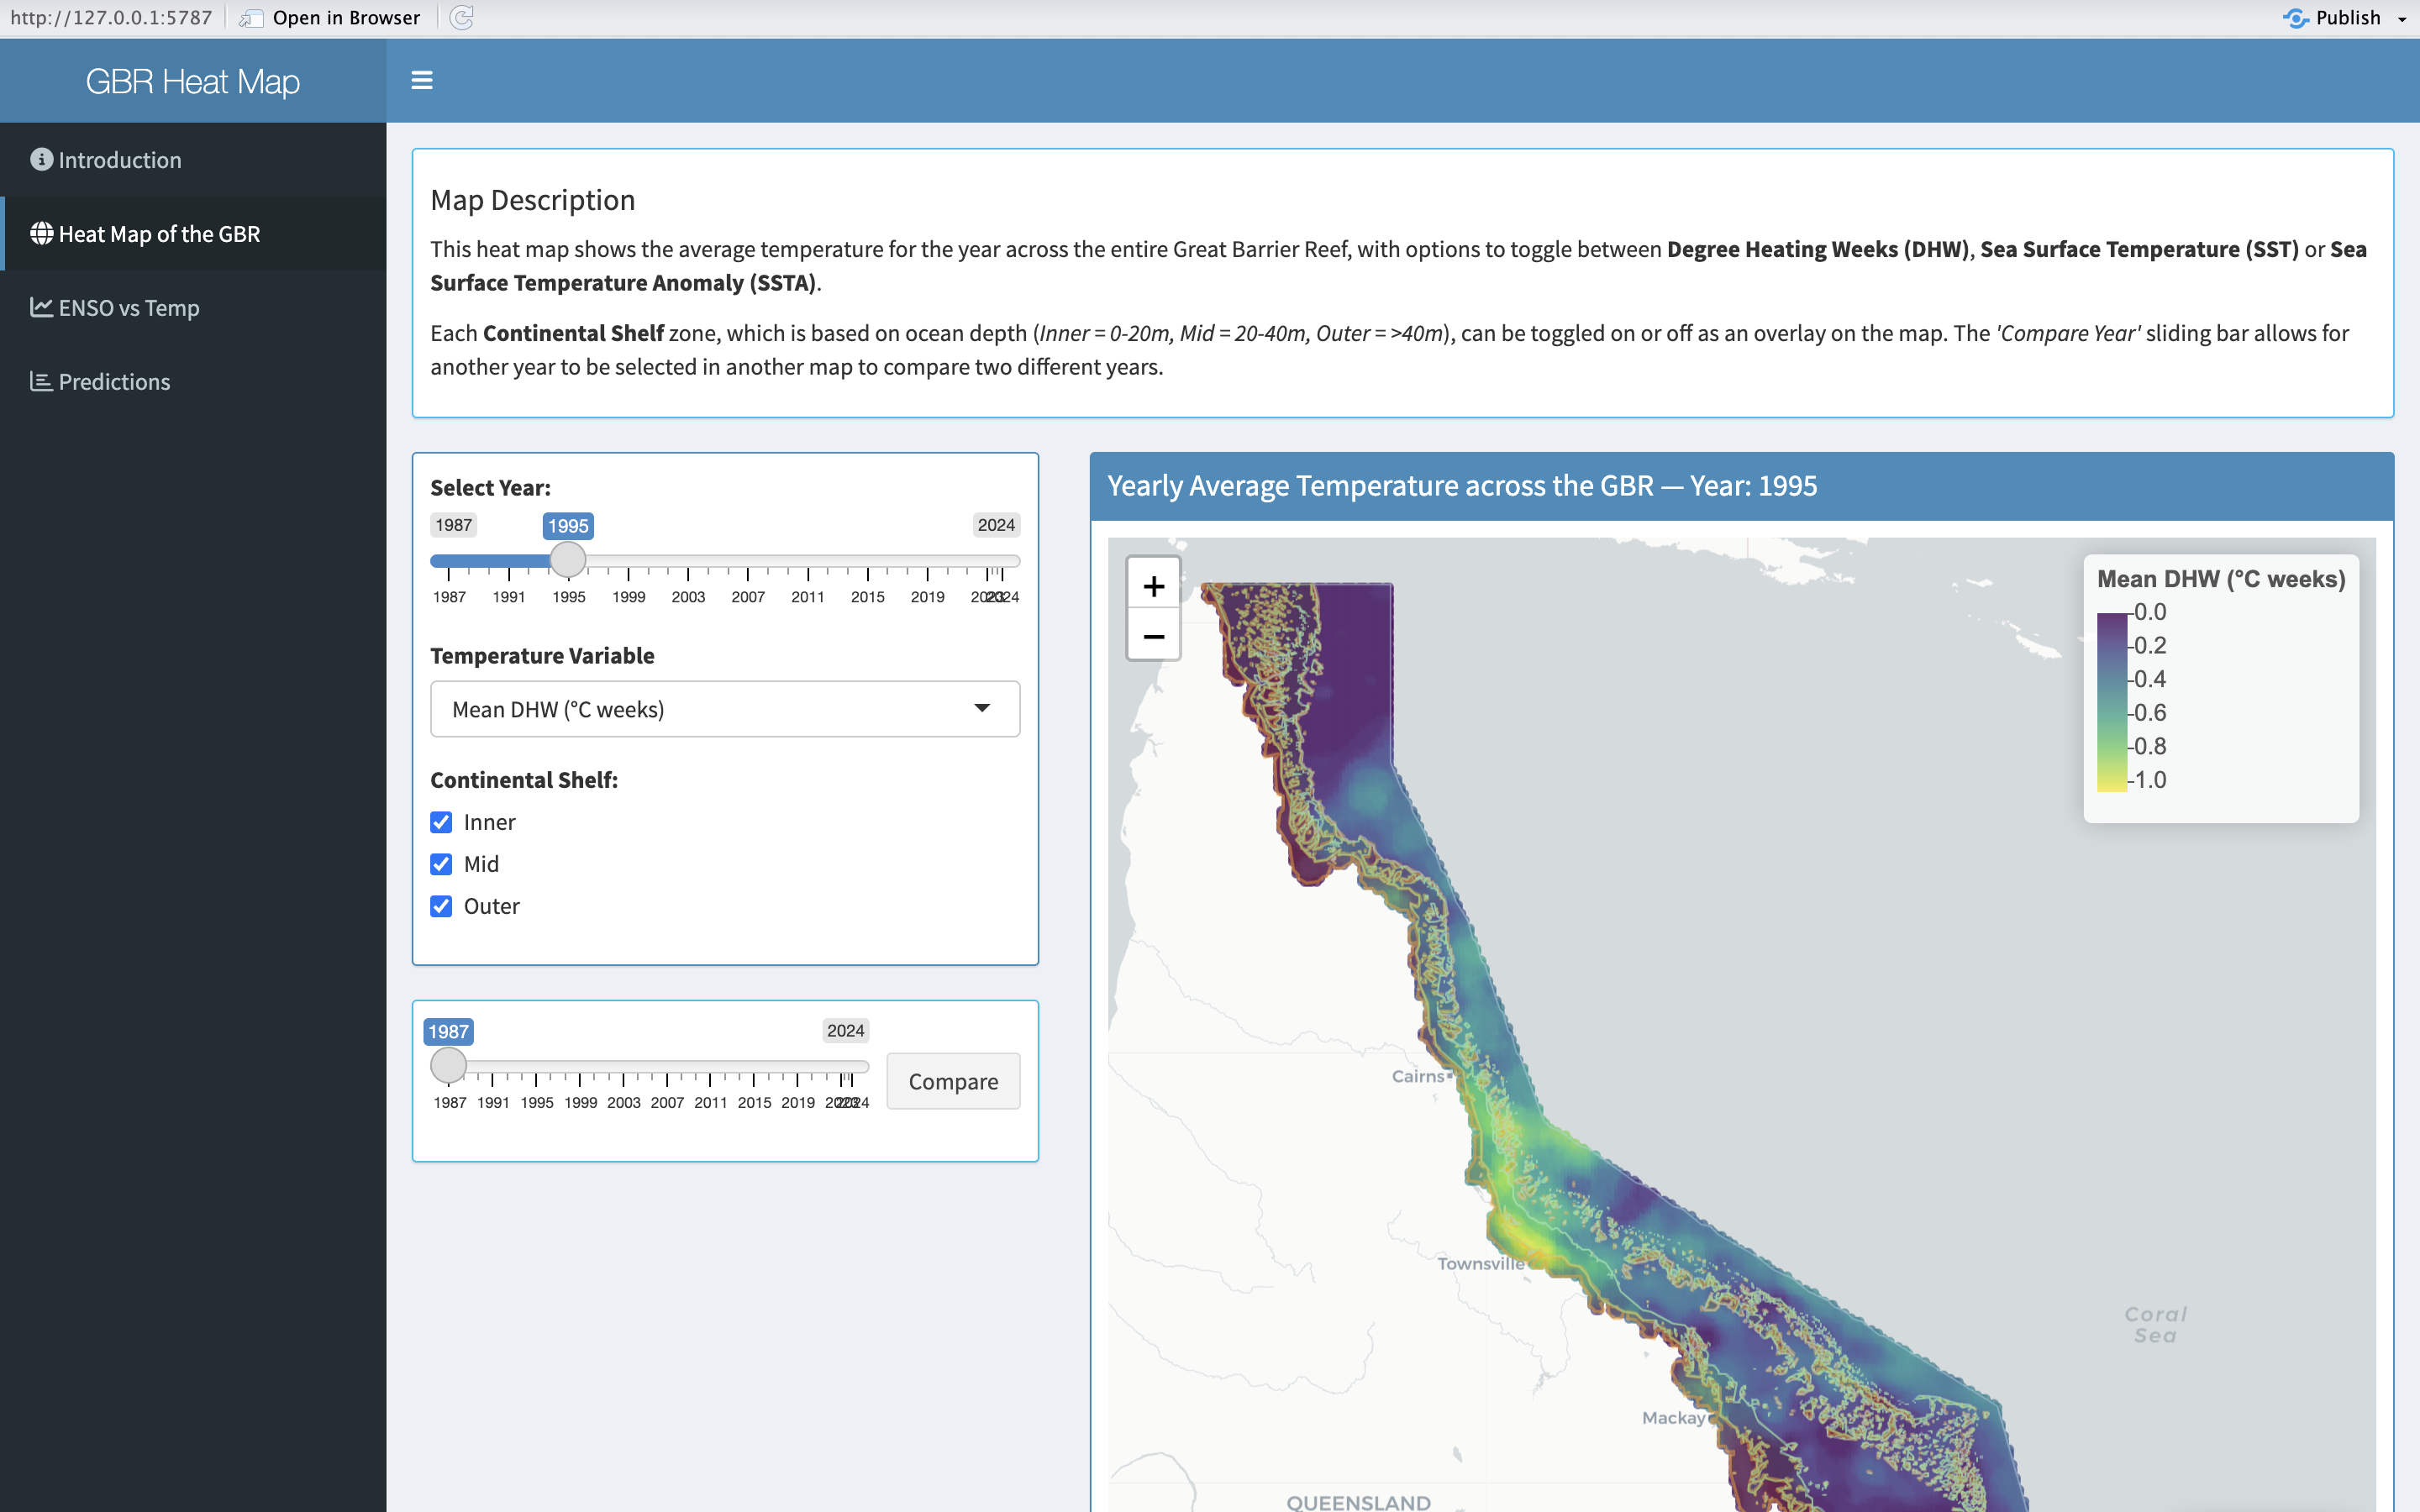
\includegraphics[width=0.5\textwidth]{report_images/shiny_map_a.png}
\end{center}

\begin{center}
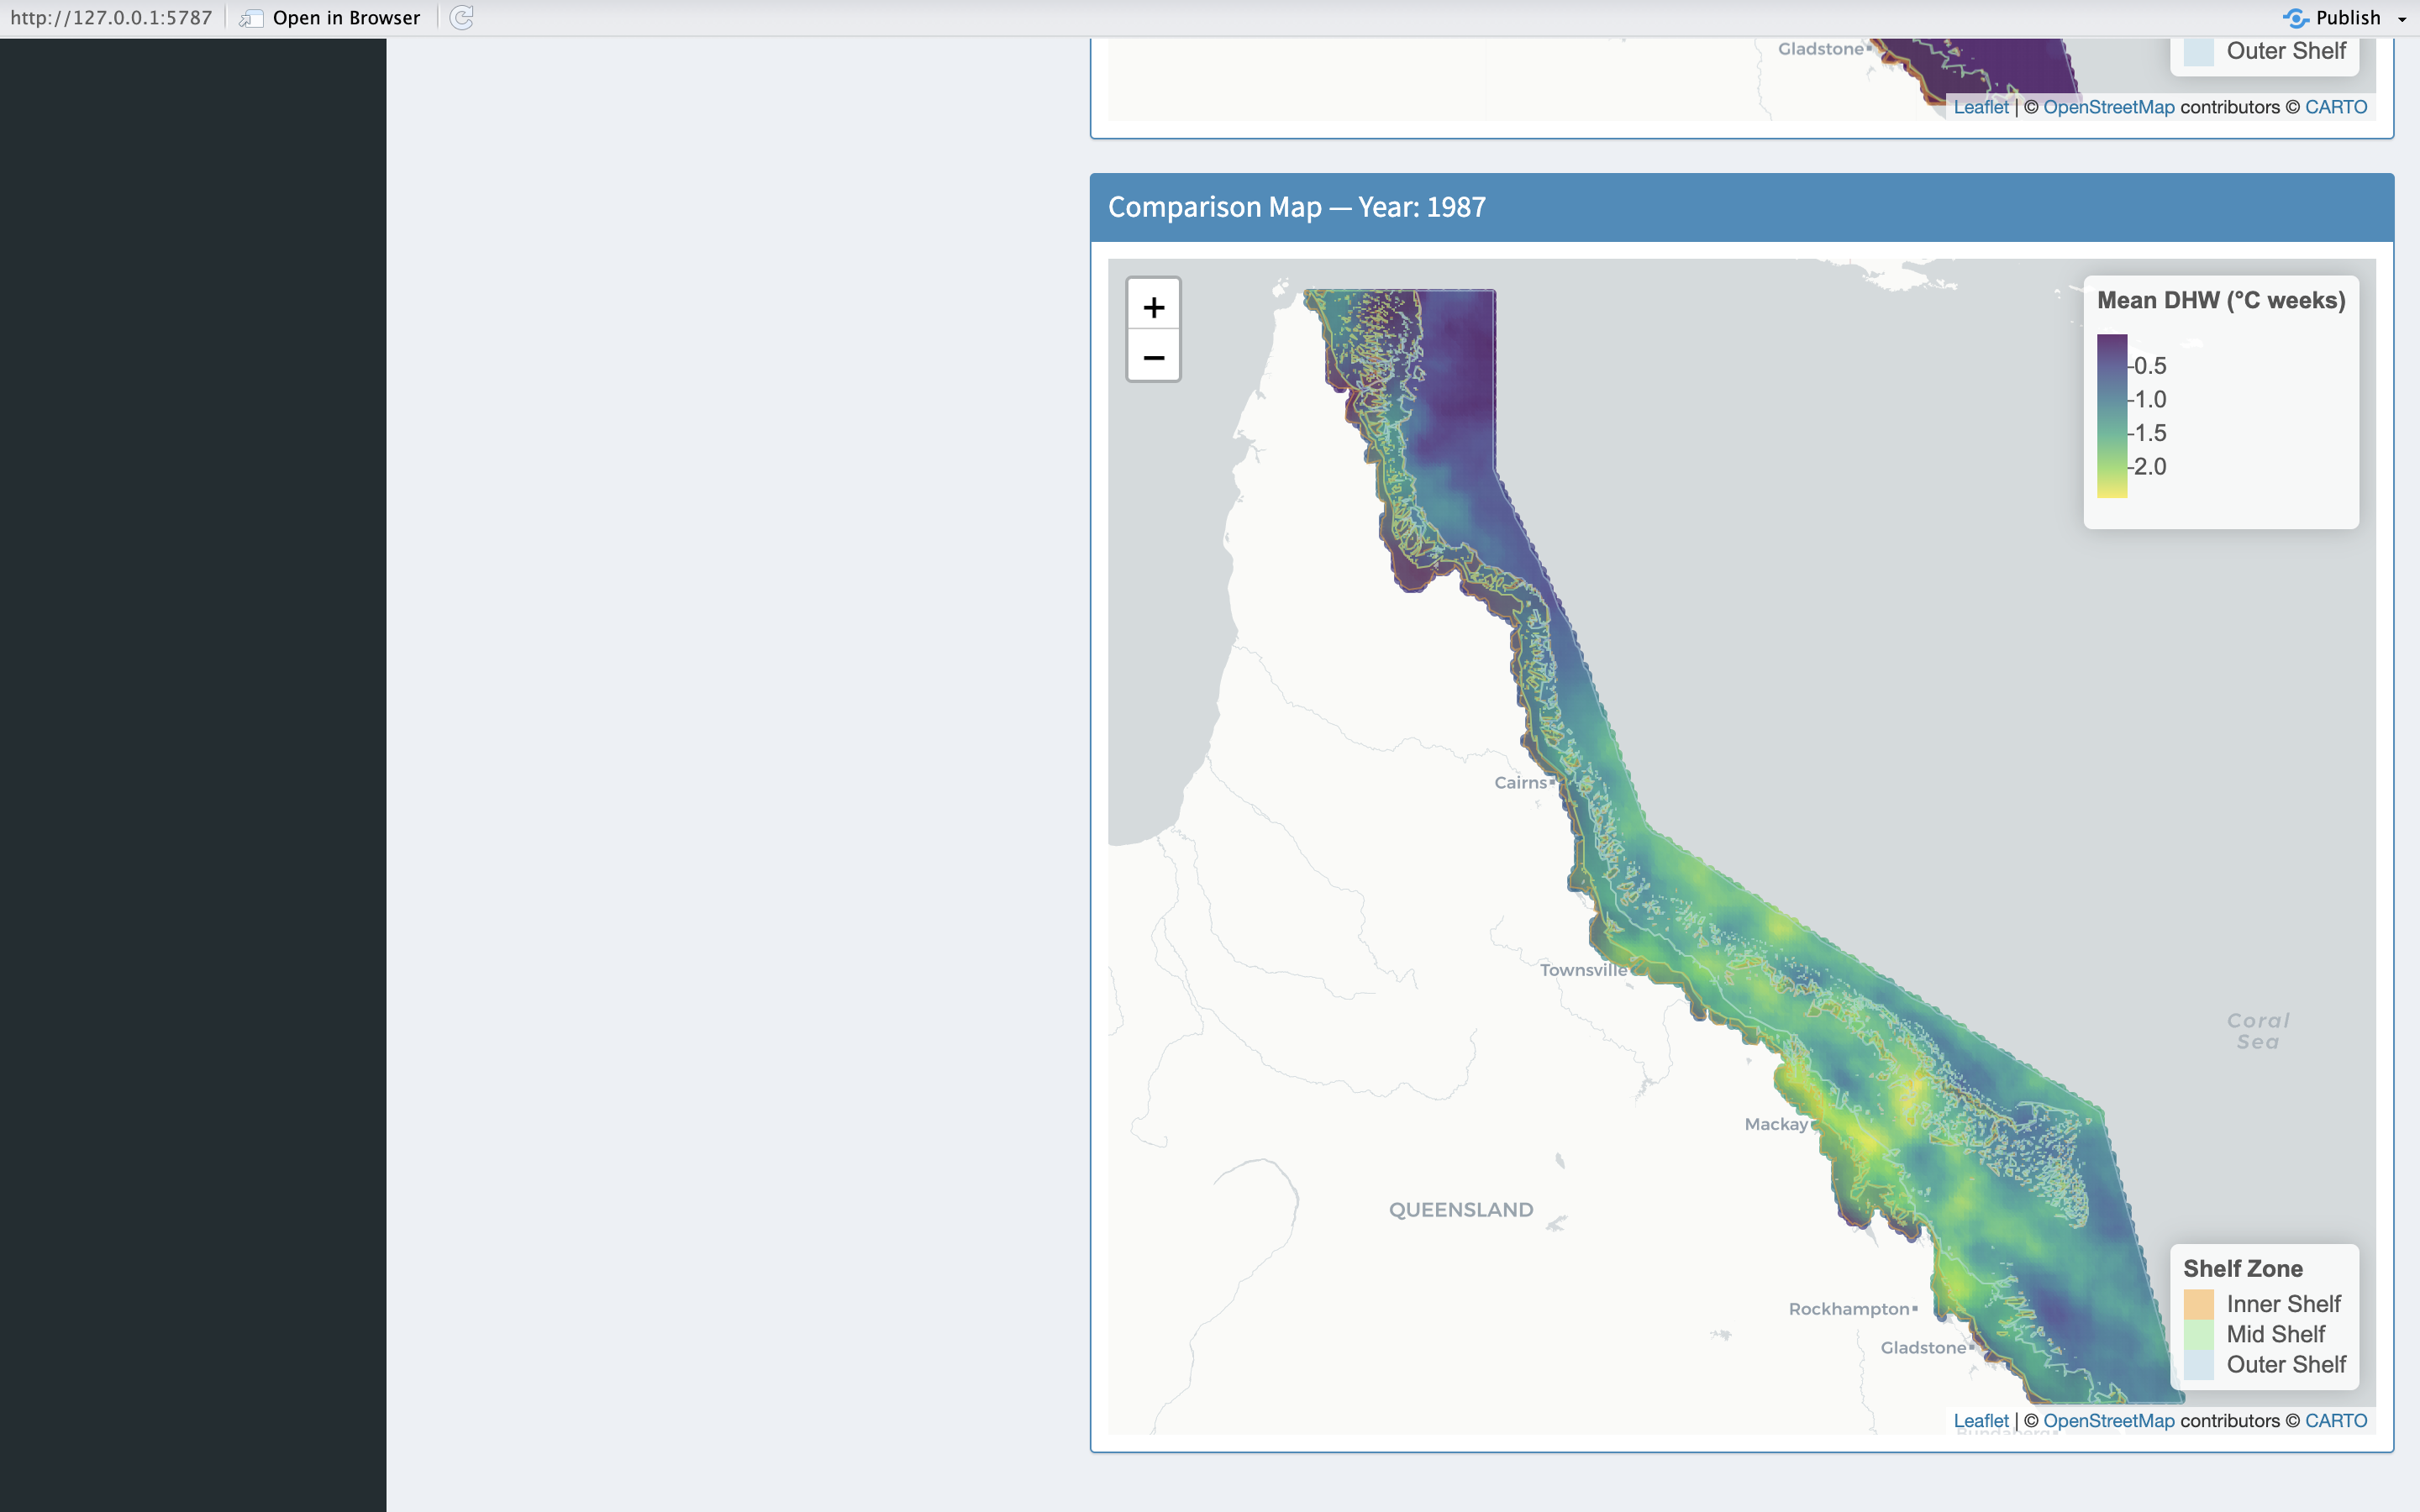
\includegraphics[width=0.5\textwidth]{report_images/shiny_map_b.png}
\end{center}

\begin{center}
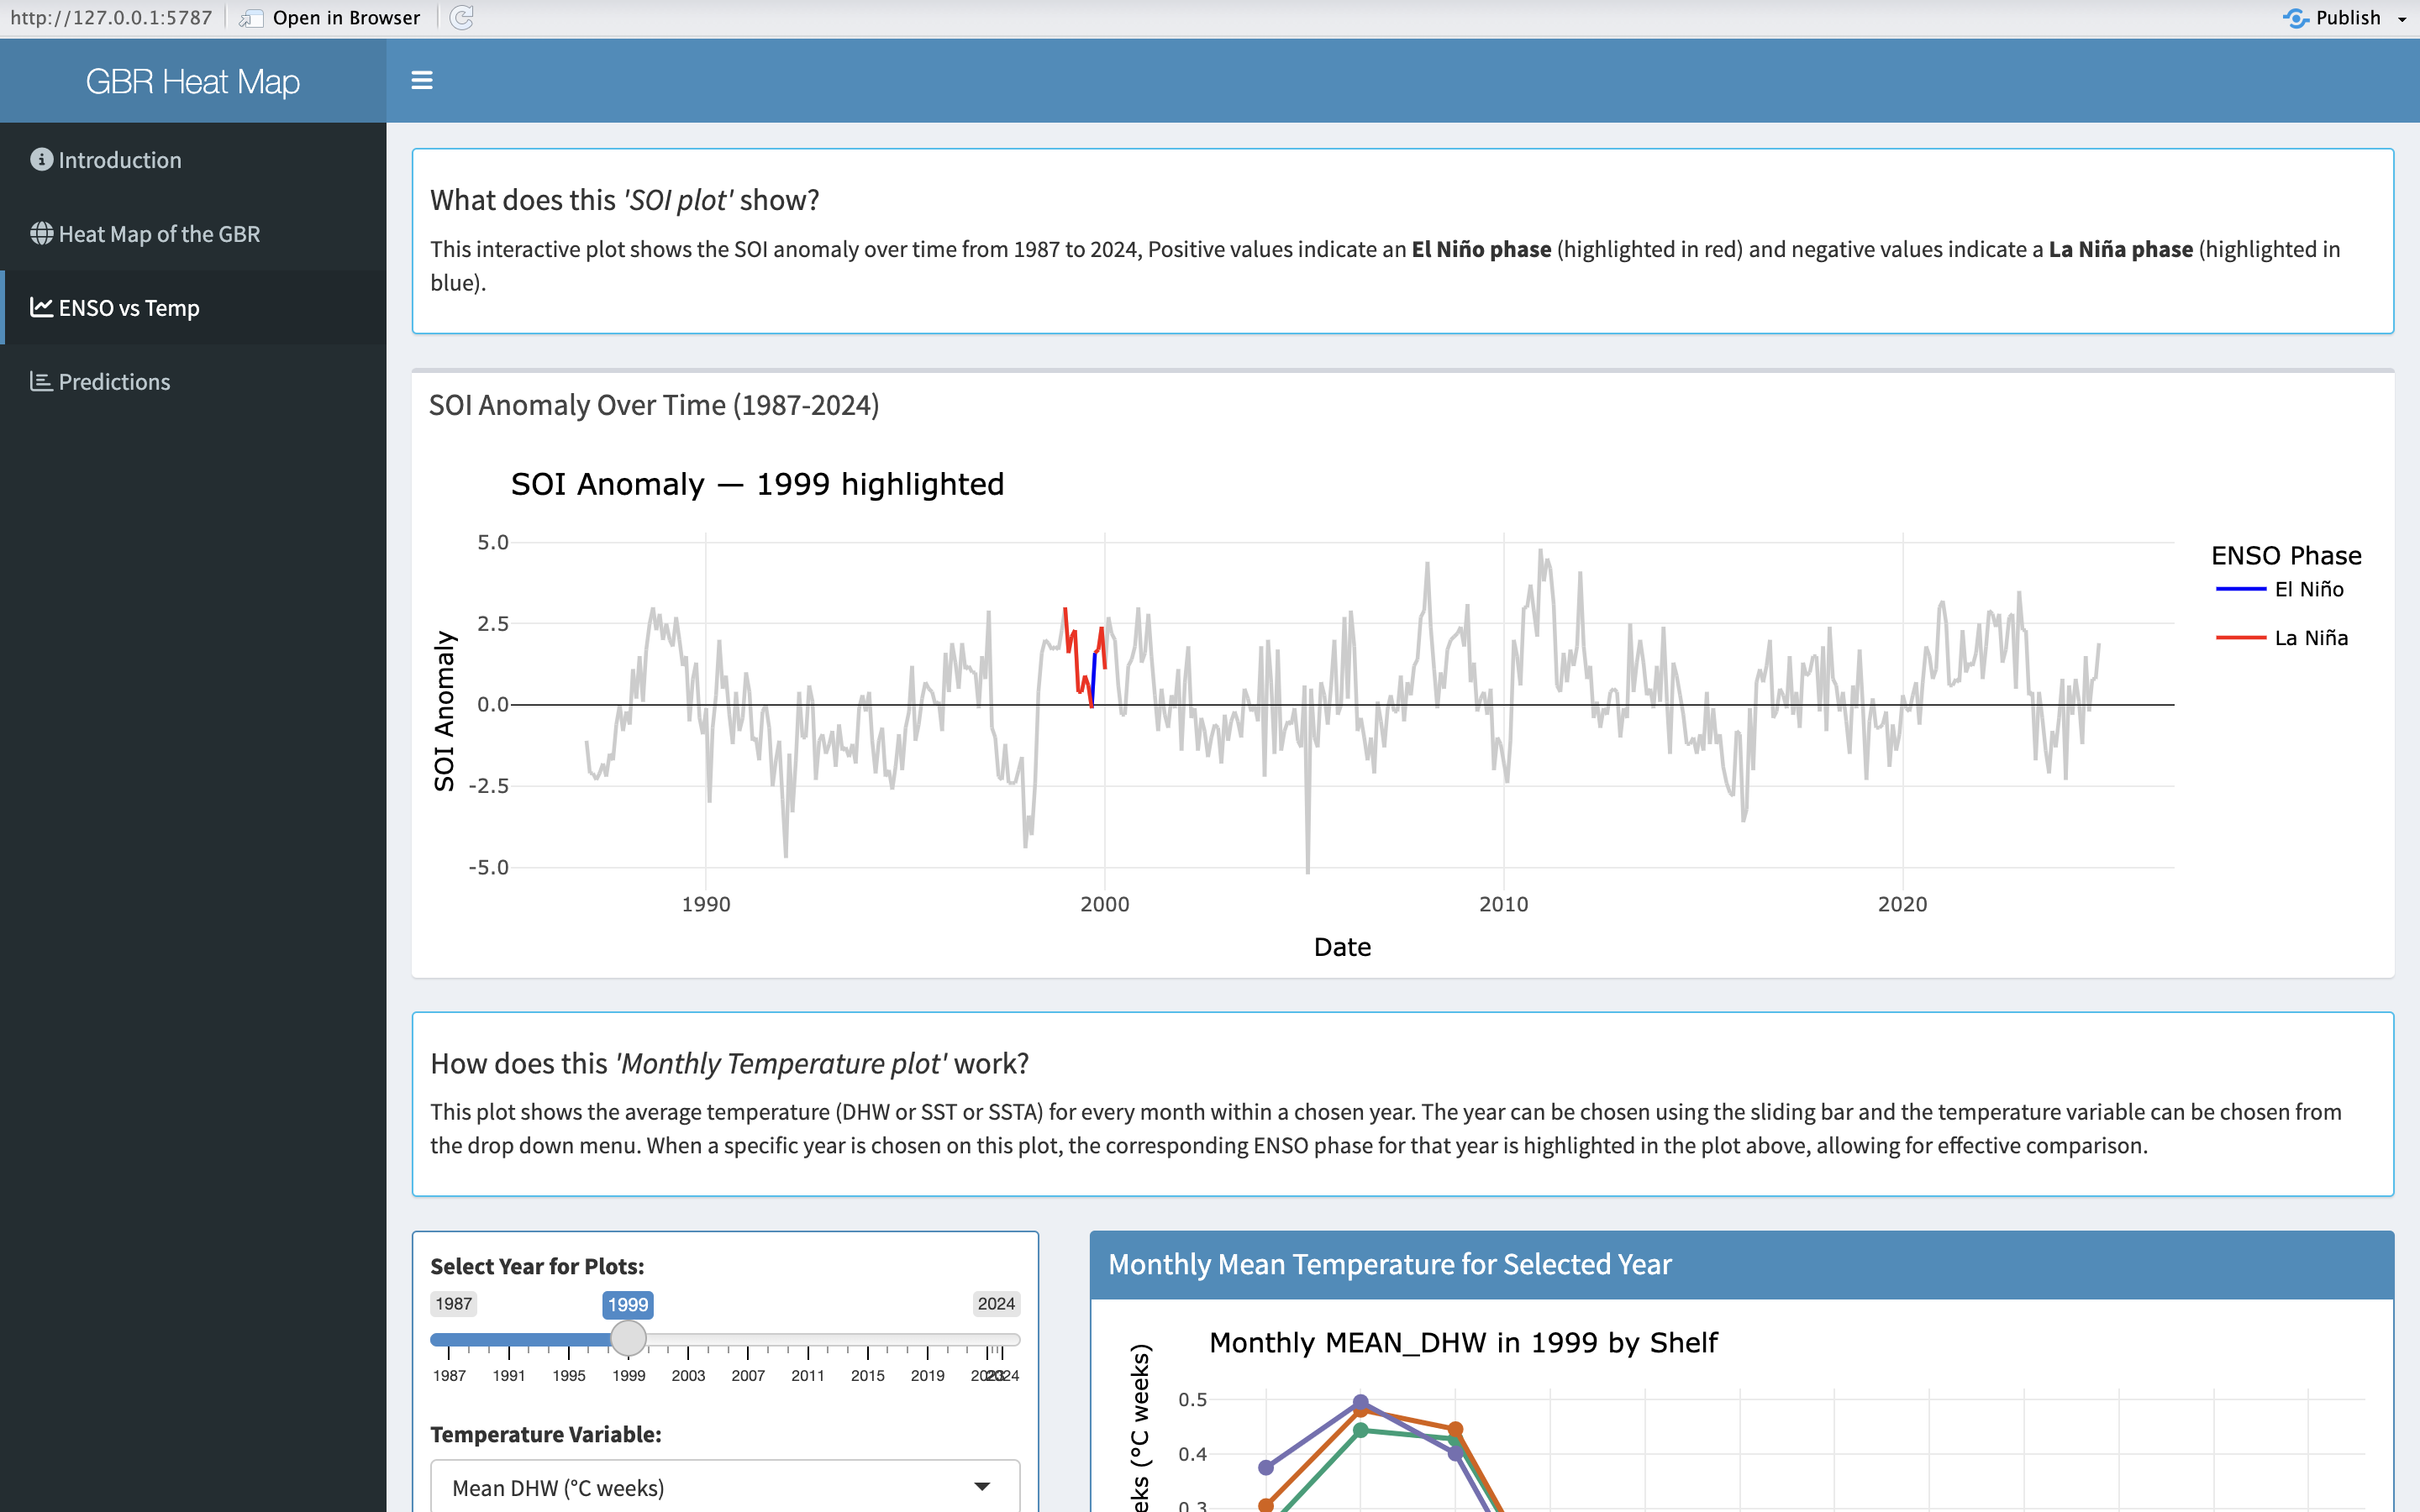
\includegraphics[width=0.5\textwidth]{report_images/shiny_enso_temp_a.png}
\end{center}

\begin{center}
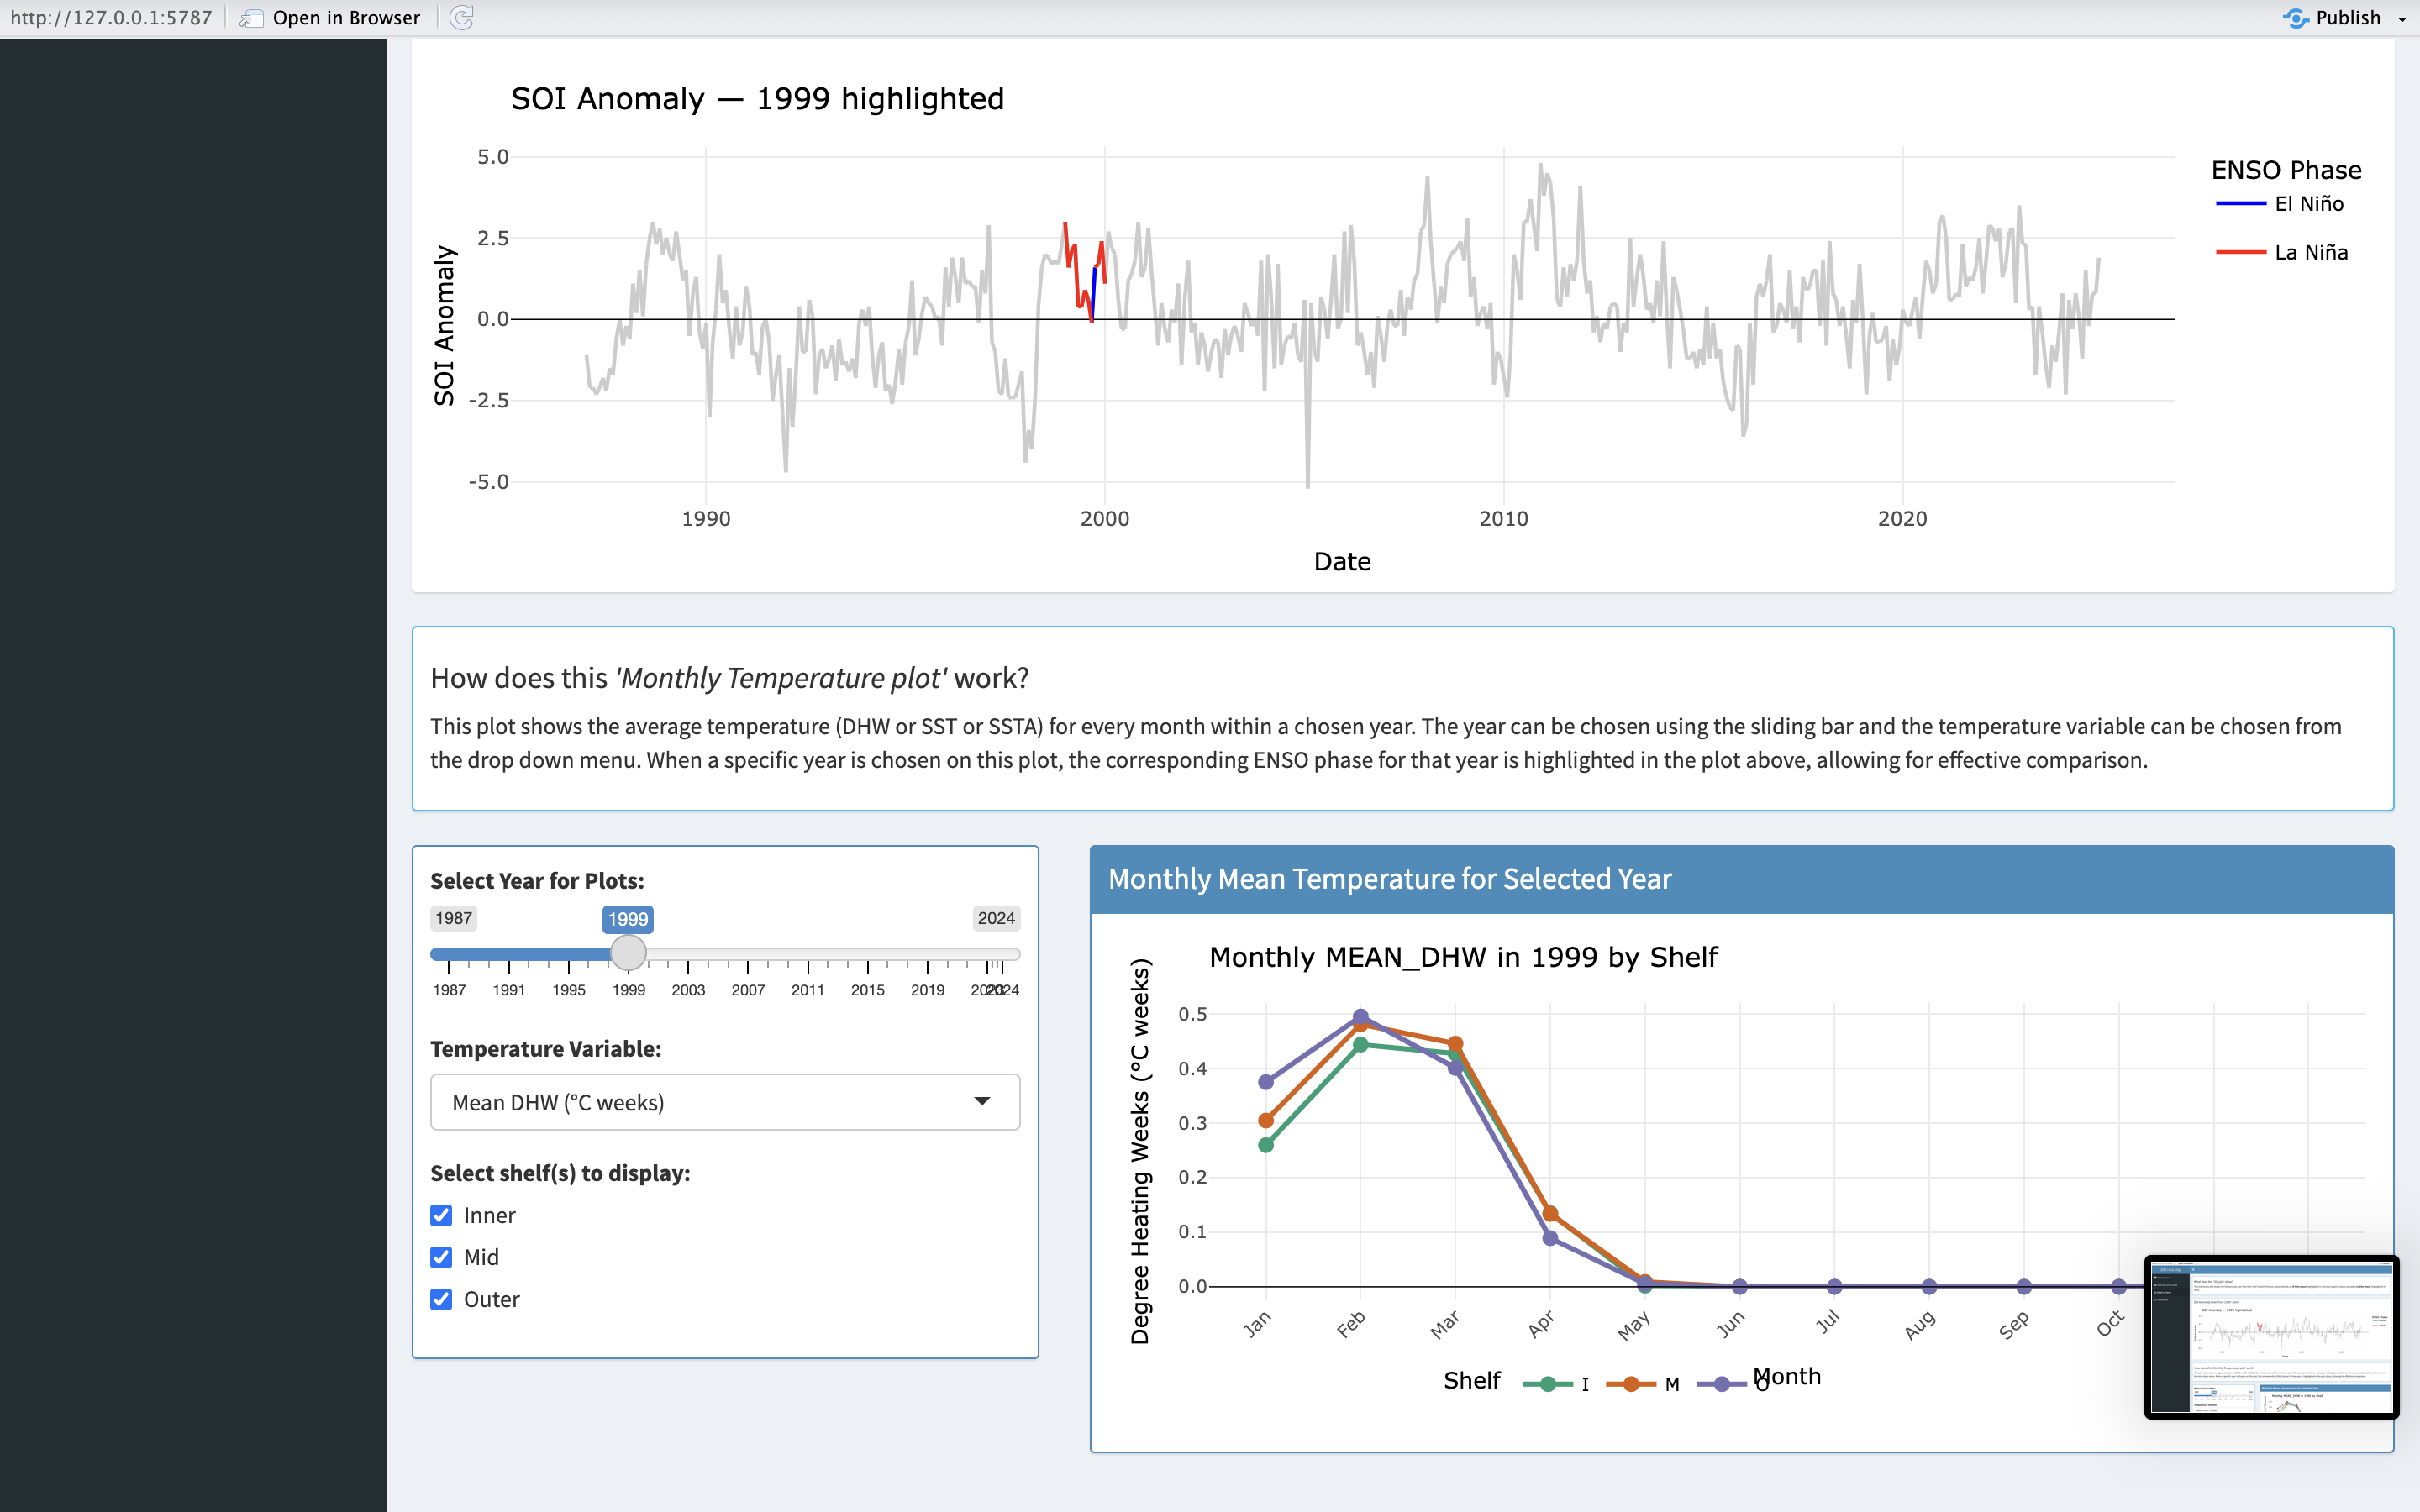
\includegraphics[width=0.5\textwidth]{report_images/shiny_enso_temp_b.png}
\end{center}

\begin{center}
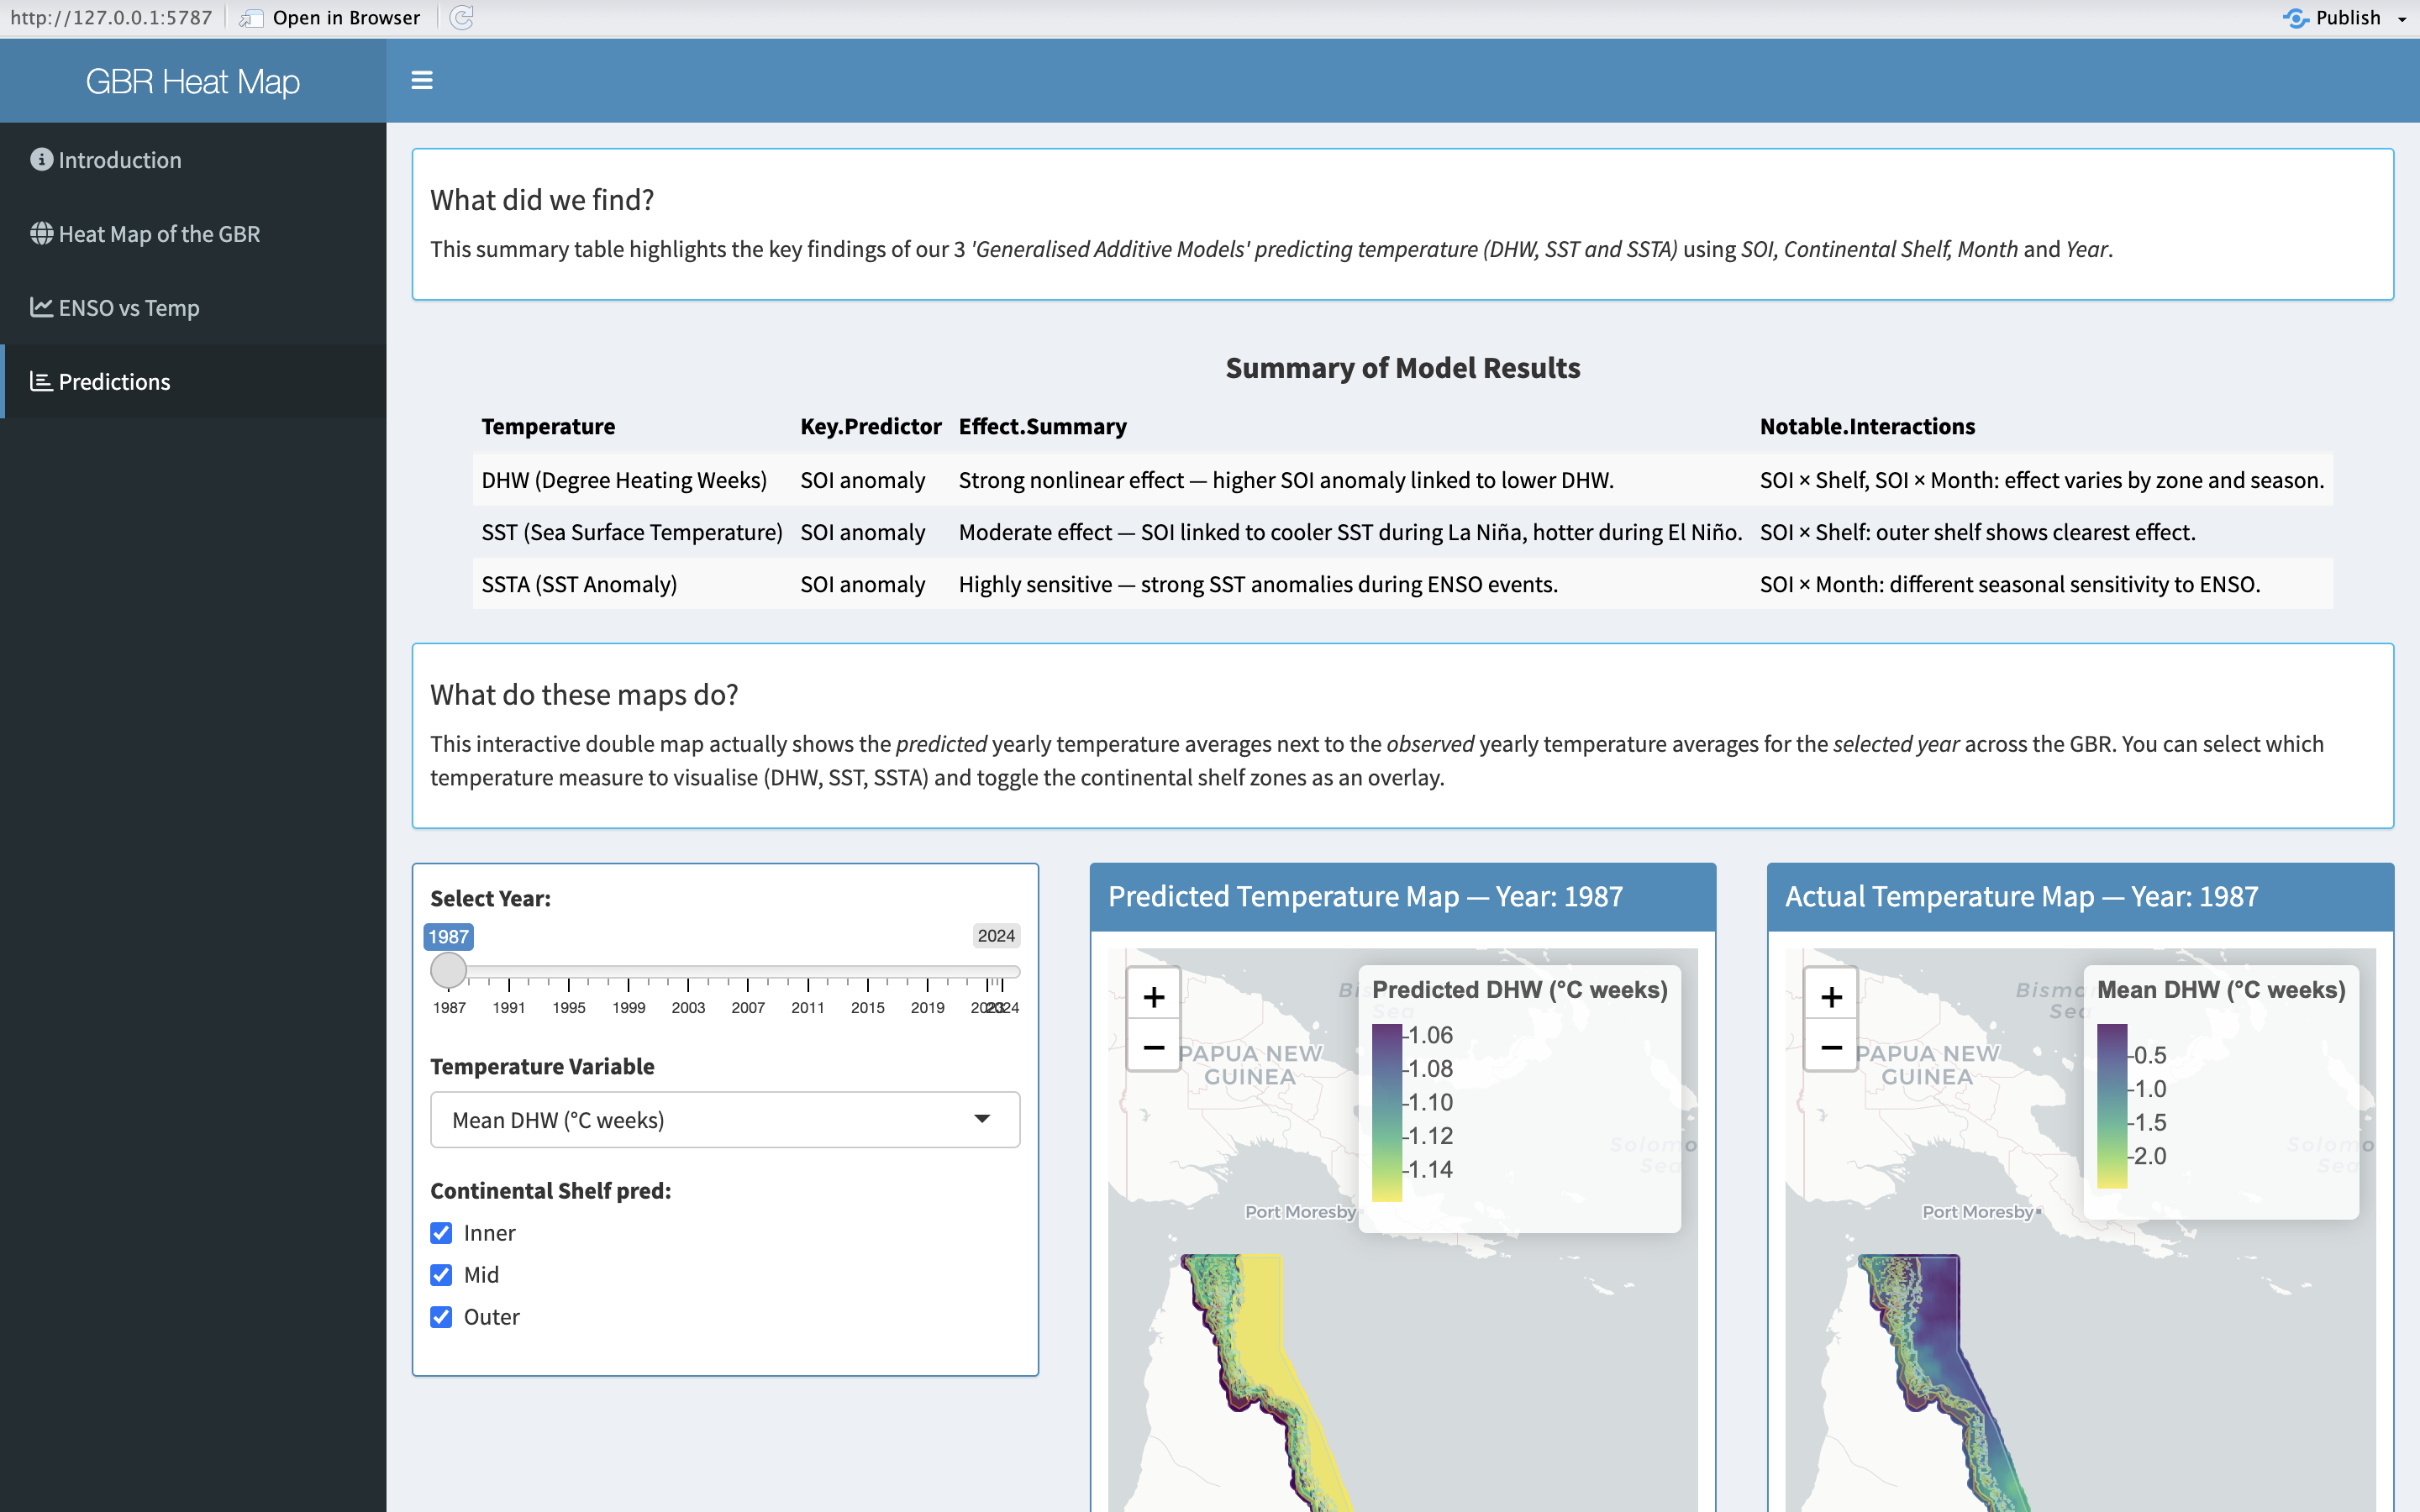
\includegraphics[width=0.5\textwidth]{report_images/shiny_predictions.png}
\end{center}

%\showmatmethods


\bibliography{pinp.bib}
\bibliographystyle{jss}



\end{document}
